\documentclass{article}
\usepackage[utf8]{inputenc}
\usepackage{graphicx}
\usepackage{hyperref}
\usepackage{float}

\title{Project EPIC - User Manual}
\author{Francois Mouton}
\date{August 2015}

\begin{document}
\newcommand{\HRule}{\rule{\linewidth}{0.5mm}}
\begin{titlepage}
\begin{center}

\includegraphics[width = 0.3\textwidth]{US_logo.png}~\\[1cm]
\textsc{\LARGE Unsolvable Solutions}\\
Client: Francois Mouton at the CSIR DSSR\\[1.5cm]
\textsc{\Large  Functional Requirements}\\[0.5cm]

 \HRule\\[0.4cm]
{ \huge \bfseries  Eavesdropping Protection in Conclave \\[0.4cm] }

 \HRule\\ 



Github link:  \url{https://github.com/Unsolvable-Solutions/Project-EPIC} \\[1.2cm]

\noindent
\begin{minipage}[t]{0.4\textwidth}

	\begin{flushleft} \large
	\emph{Members:}\\
		Edwin Fullard  \\
		Jaco Bezuidenhoudt \\
		Jandre Coetzee\\
		Maret Stoffberg\\
		Ryno Pierce\\
	\end{flushleft}
\end{minipage}%
\begin{minipage}[t]{0.4\textwidth}
\begin{flushright} \large
	\emph{Student Number:} \\
		12048675 \\
		11013878 \\
		 10693077 \\
		 11071762 \\
		 12003922\\
	\end{flushright}
\end{minipage}

\vfill


% Bottom of the page




\end{center}
\end{titlepage}




\tableofcontents



\newpage
\section{System Overview}
The purpose of the EPIC(Eavesdropping protection in Conclave) project is to protect the confidential information discussed in a meeting. This is achieved by making sure the users phone or tablets data, Wifi and GSM are switched off during the meeting.

This EPIC project consist of a server, Android application, NFC Node, Website, and an Intel Edison device. 
The Android device is held over the NFC Node. The NFC then sends a request to the server via the Edison to enter the meeting. The server then responds with access granted or not. If access is granted, the user may the proceed to the meeting and the data, wifi and GSM of the device is turned off. When the user then exists the meeting, the device is held over the Node again and the previous state is restored. 
The user may use the website to register, create a new meeting and to query the attendance log of a past meeting.

For the purpose of testing the EPIC project, a Malware application and server are also developed. The Malware can be used to eavesdrop on unsuspecting victims. 



\newpage
\section{System Configuration}

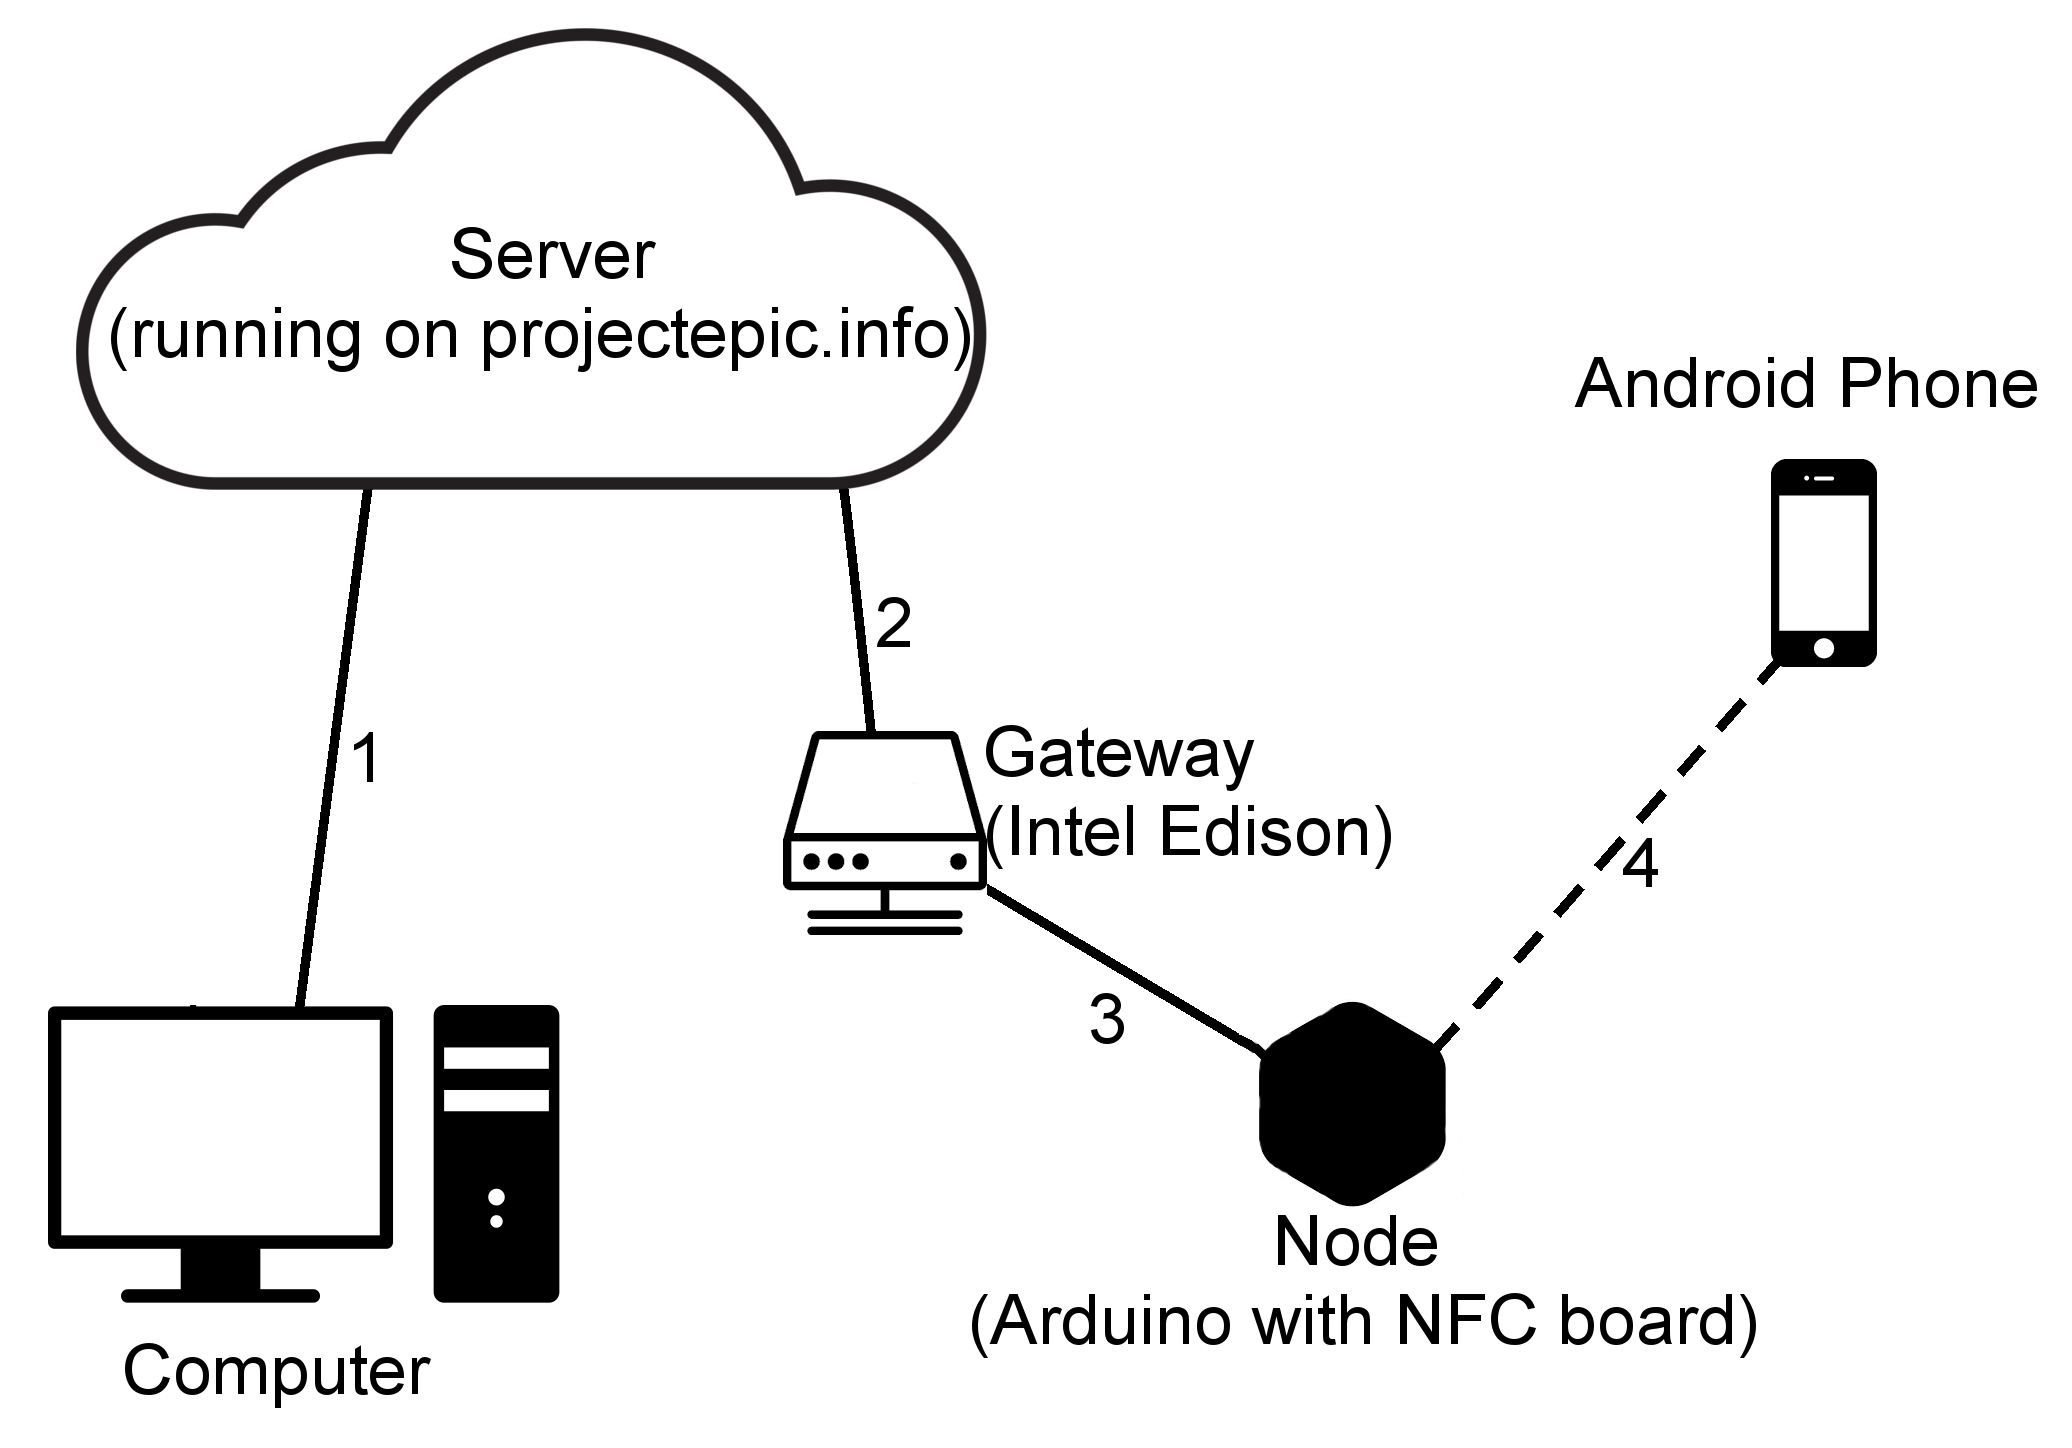
\includegraphics[width=12cm, height=8.5cm]{SystemLayout}
\begin{enumerate}
\item Connects through the Internet via a web browser.
\item Connects to the server via Wifi. It relays the data from the Node to the Server and vice versa.
\item Connects using a cable. It sends the users' information, obtained from the phone via NFC, to the Gateway. And transmits results, received from the Gateway, via NFC to the Phone.
\item Communicates using NFC. The phone sends the Users' email address and password, and then the Node sends back the Servers' response.
\end{enumerate}



\newpage
\section{Installation}

\subsection{Android Application}
\begin{enumerate}
\item Copy the apk file name EPICApp over to your device.
\item Locate the file on your device and tap on the file.
\item A list of permissions will pop-up that the application needs in order to function. Click on the install option.
\item The application is now ready to use.
\end{enumerate}

\subsection{Node}
\begin{enumerate}
\item Download the Arduino IDE for your respective OS.
\item Clone the GitHub repository to get the code.
\item Add all the libraries to the Arduino IDE.
\item Plug in the Node and upload the code through the IDE.
\end{enumerate}

\subsection{Intel Edison}
\begin{enumerate}
\item Download the Intel Edison Standalone driver
\item Use Putty (Windows) or Screen (Linux) to attach to the serial port at a 115200 BAUD rate
\item Clone the GIT Repo and cd into the EPICEdison directory. Run npm install and then after it's done run npm start
\item The Intel Edison is now ready to use.
\end{enumerate}

\subsection{Server}
\begin{enumerate}
\item Install node and npm on your server
\item Clone the GIT repo and cd into the EPICServer directory. Run npm install and npm start to start the server
\item Make sure port 1337 is open in your firewall or that your webhost application point to localhost:1337
\item Enjoy the server application
\end{enumerate}

\subsection{EPIC Malware}
\subsubsection{Android Malware Application}
\begin{enumerate}
\item Copy the apk file name EPICMalware over to your device.
\item Locate the file on your device and tap on the file.
\item A list of permissions will pop-up that the application needs in order to function. Click on the install option.
\item The application is now ready to use.
\end{enumerate}
\subsubsection{Java Malware Server}
\begin{enumerate}
\item Make sure a minimum version of Java 7 is running on your system.
\item Locate the EPICMalwareServer.jar file on your system.
\item Execute the the file with the following command "java -jar EPICMalwareServer.jar"
\item Follow the on-screen instructions.
\end{enumerate}

\newpage
\section{Getting Started}

\subsection{Android Application}
\begin{enumerate}
\item To get started, first navigate to to application shortcut name EpicApp and open it.
\item If NFC is turned off the application will open the settings screen shown in the next step. If NFC is turned on go to step 4.
\item {If NFC is turned off the following screen will be presented:
\begin{figure}[H]
\center
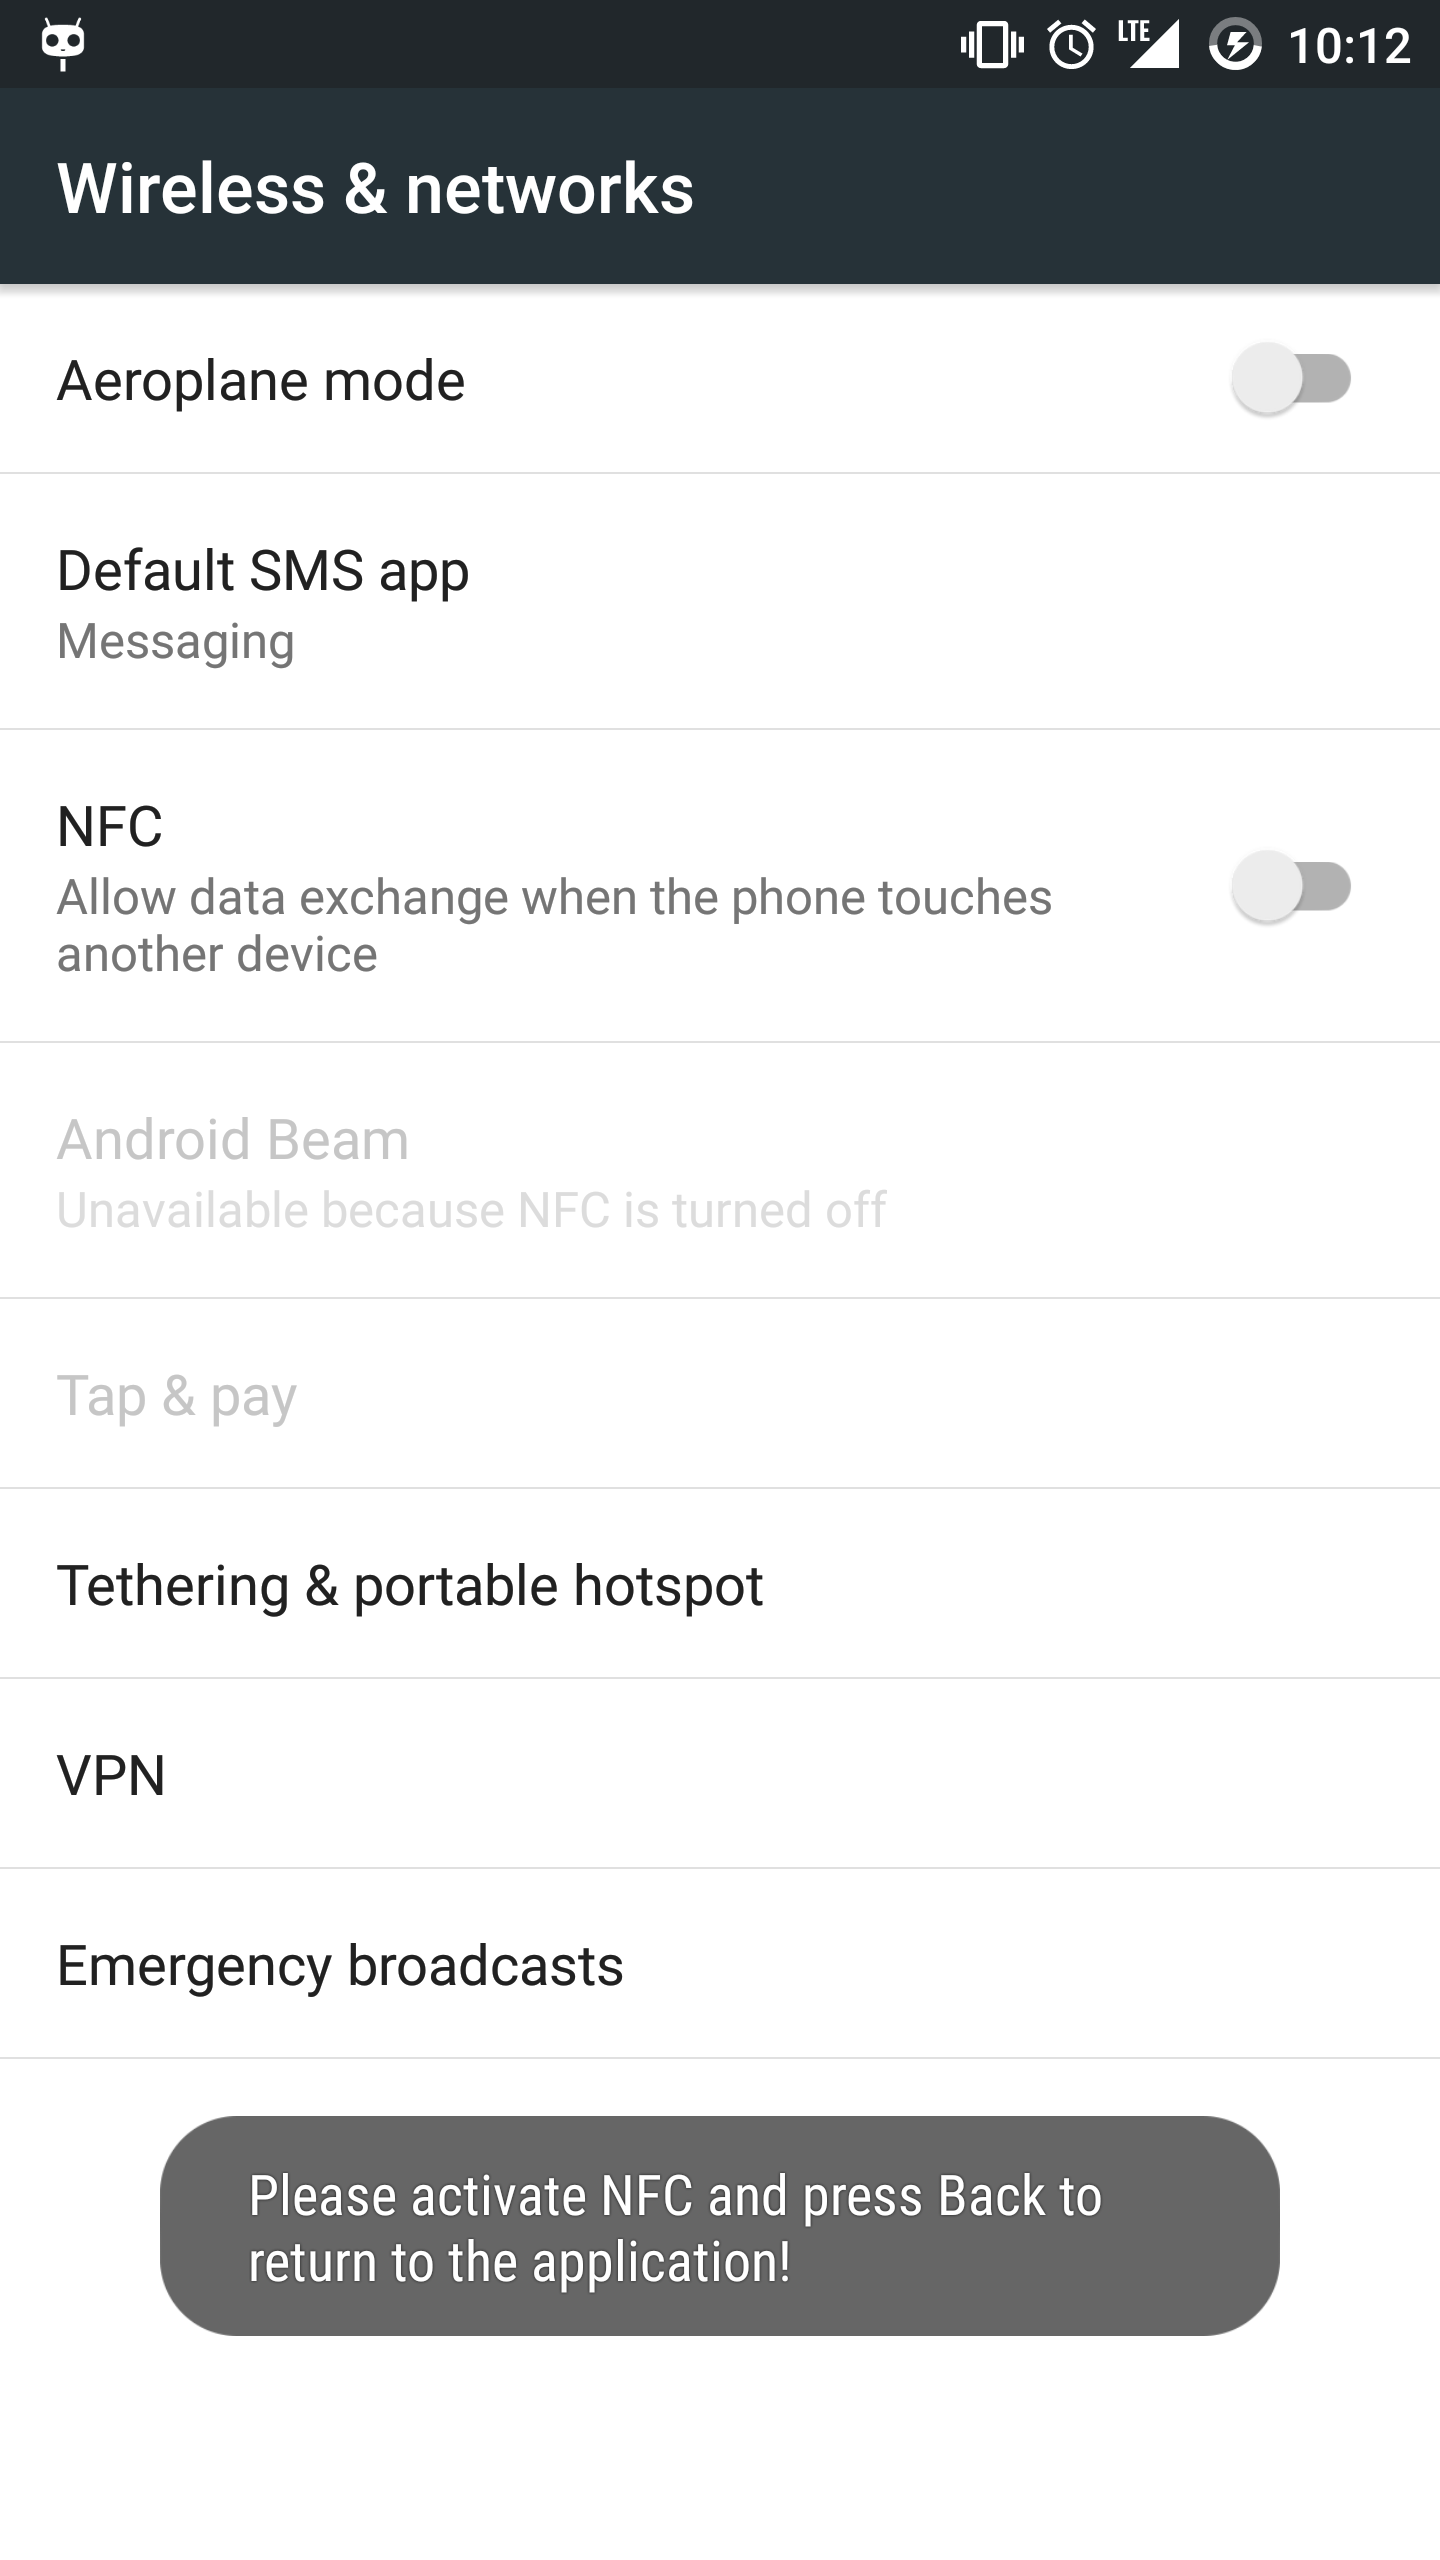
\includegraphics[width=5cm, height=6cm]{Settings}
\caption{NFC Settings}
\label{fig:my_label}
\end{figure}}
Turn the NFC on by clicking on the slider. After it is turned on press the back button.
\item{ On the next screen there is an edit box with the text \textit{New Employee ID}. Click on it and type in the registered ID given to you and press the done or check mark key.
\begin{figure}[H]
\center
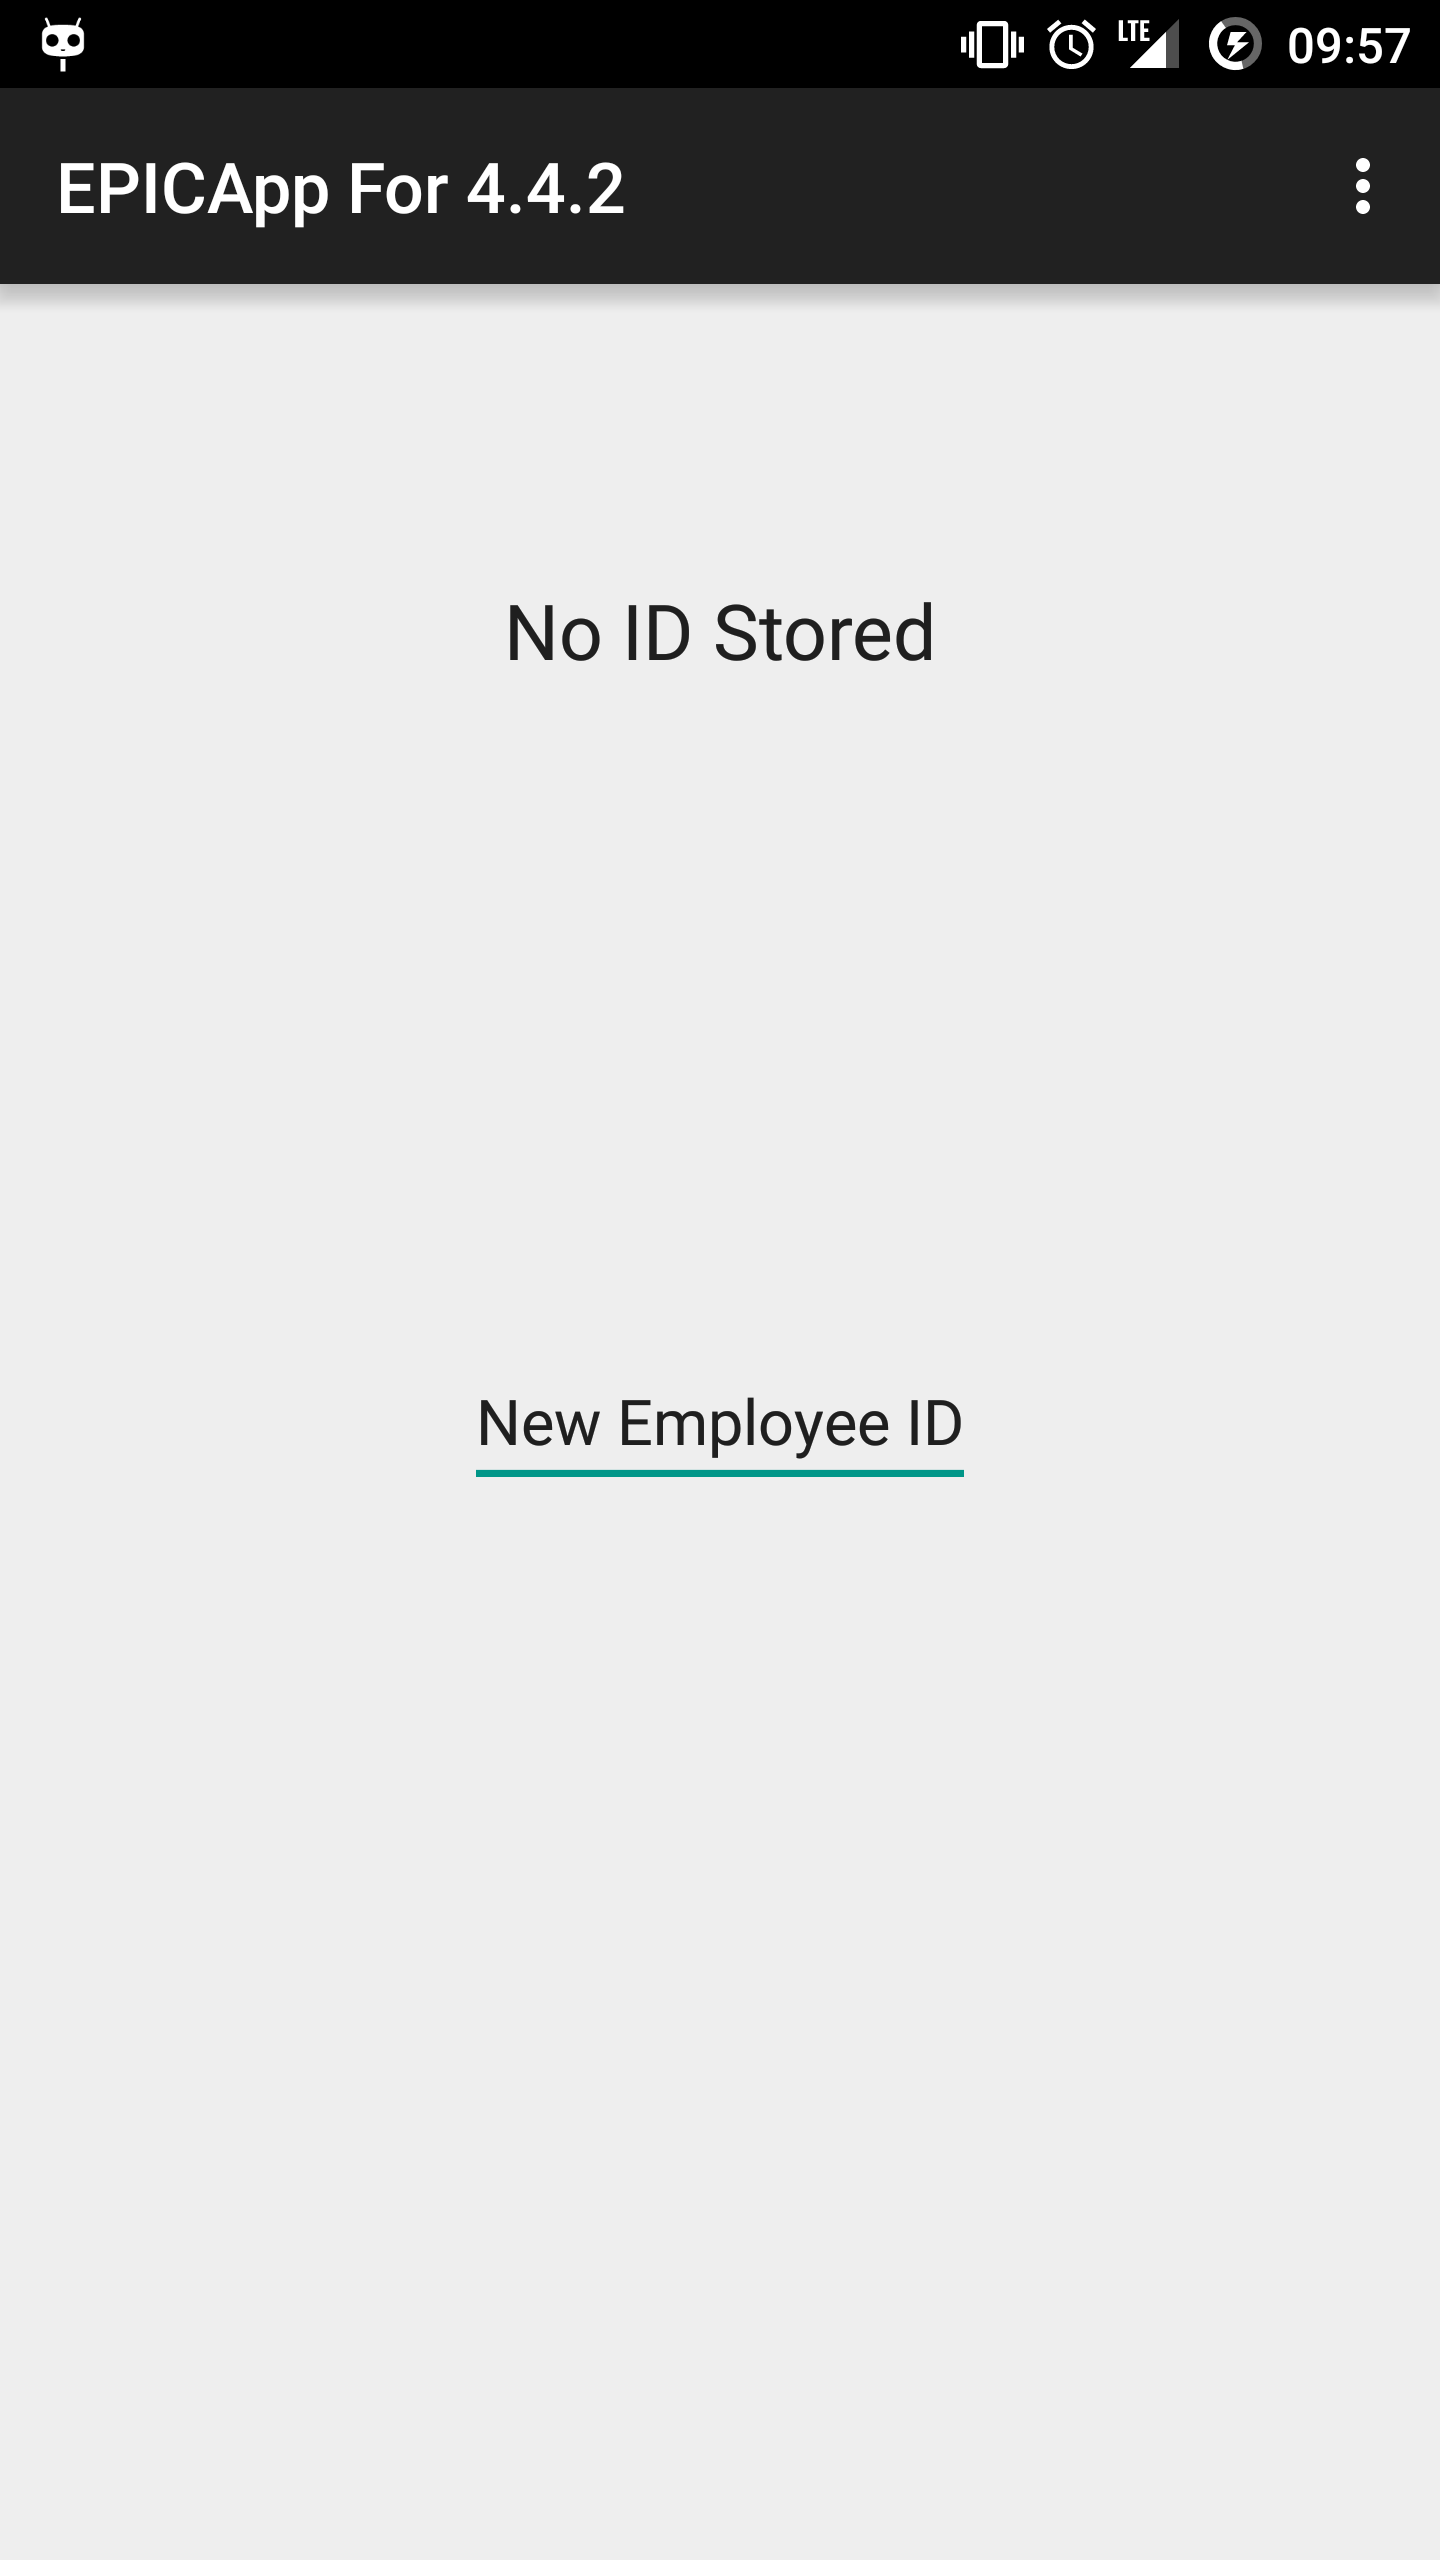
\includegraphics[width=5cm, height=6cm]{firstOpen}
\caption{Application's first use}
\label{fig:my_label2}
\end{figure}}
\item You will notice the \textit{No ID Stored} text change to your ID that you typed in. This means that the application is now ready to be used to enter the meeting room.
\end{enumerate}

\subsection{Node}
Connect the Node to the Gateway (Intel Edison) and check that the lights are Orange and Yellow strips running across.

\subsection{Website}
Open the website \url{projectepic.info} in your favourite browser.

\subsection{EPIC Malware}
\subsubsection{Java Malware Server}
To use the EPICMalware application you first need to start the malware server.
Please refer to the installation of the EPICMalwareServer to start the server.
There are two options for using the malware server, the server can control the recording or the Android application can be used to control the recording. 
\begin{figure}[H]
\center
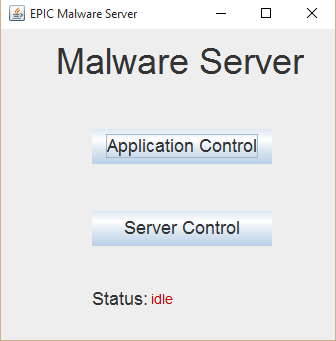
\includegraphics[width=8cm, height=8cm]{MalwareScreenshots/AppStart}
\caption{Malware Server main screen}
\label{fig:my_label5}
\end{figure}
\subsubsection{Android Malware Application}
\begin{enumerate} 
\item To get started, first navigate to to application shortcut named Eavesdrop and open it.
\item If application control was selected on the server the start recording and stop recording buttons can be used to interact with the server.
\end{enumerate}
\begin{figure}[H]
\center
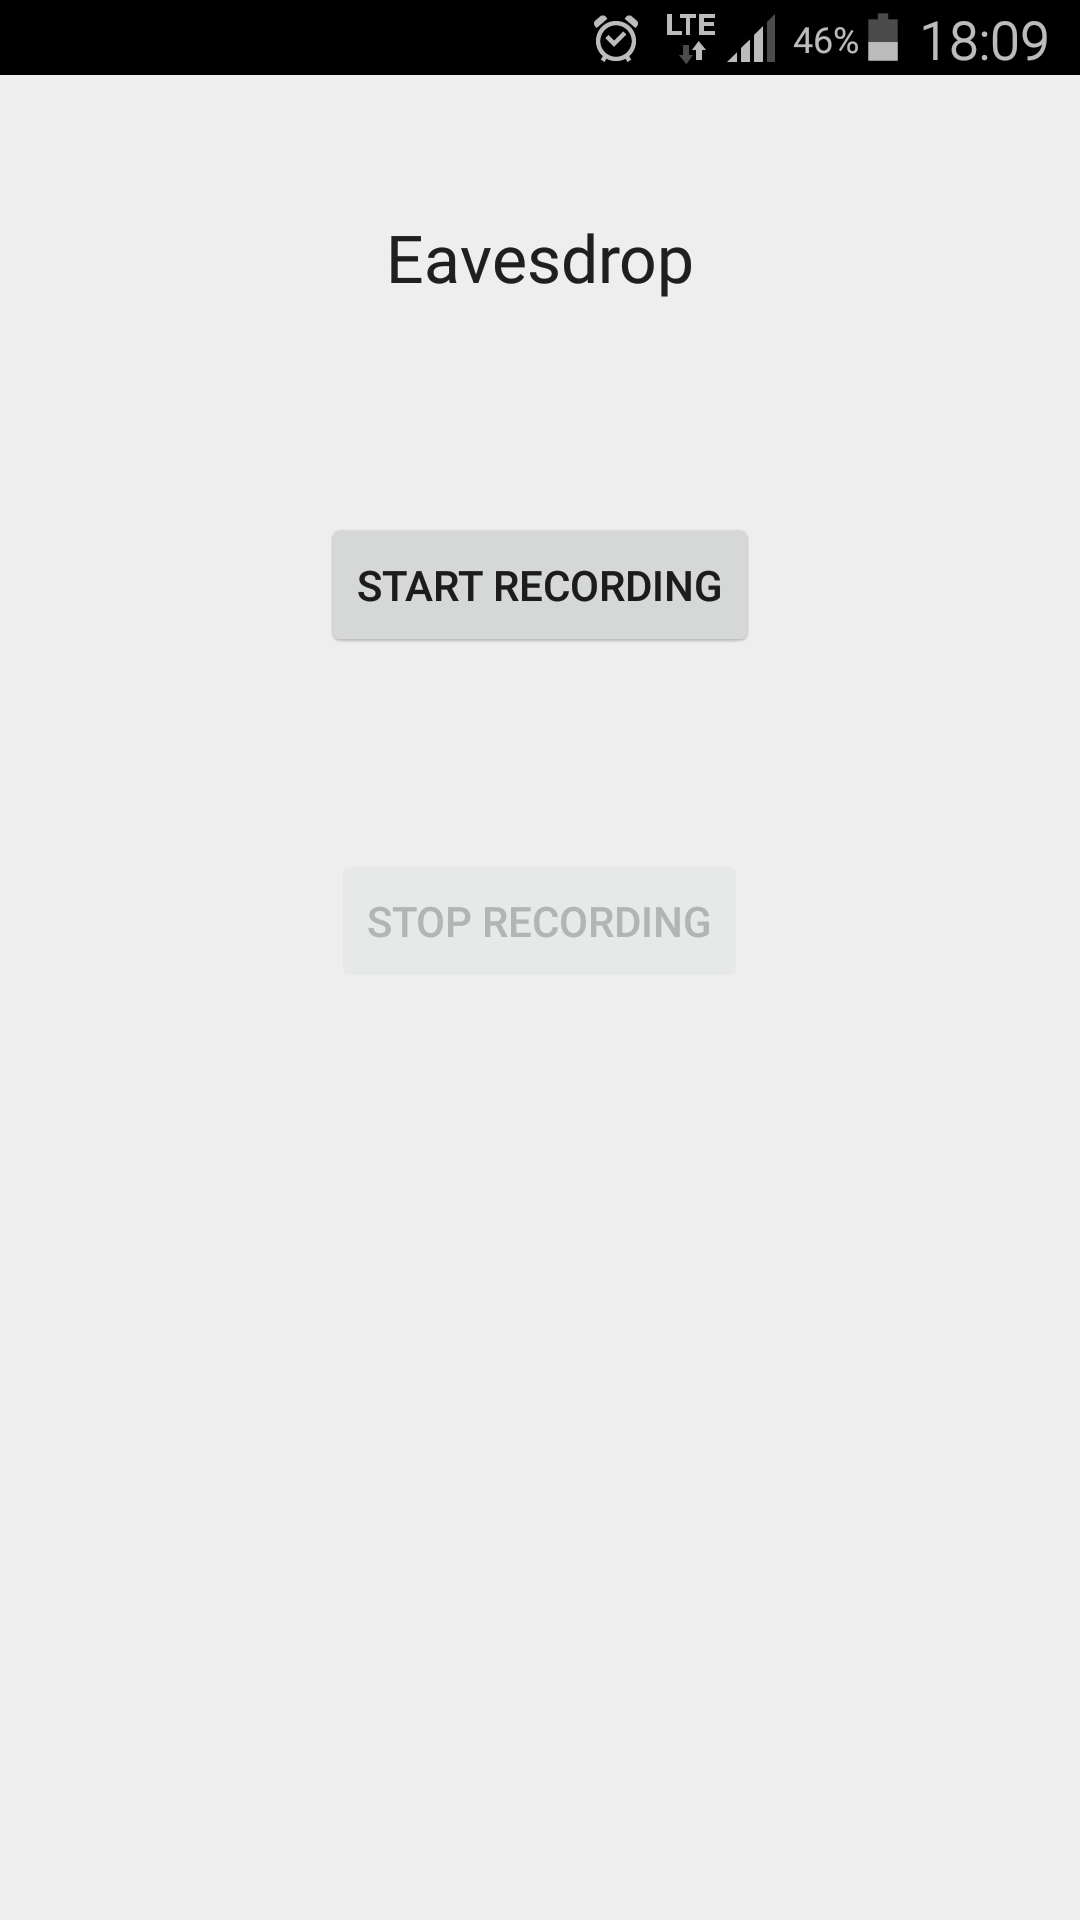
\includegraphics[width=5cm, height=6cm]{MalwareScreenshots/StartRecording}
\caption{Android malware application main screen}
\label{fig:my_label6}
\end{figure}





\newpage
\section{Using The System}

\subsection{Android Application}
To use the device with the application follow the following steps:
\begin{enumerate}
\item Bring the android device towards the entrance or exit node.
\item {After the node has flashed red or green the application will flash red or green as seen in the following images:
\begin{figure}[H]
\center
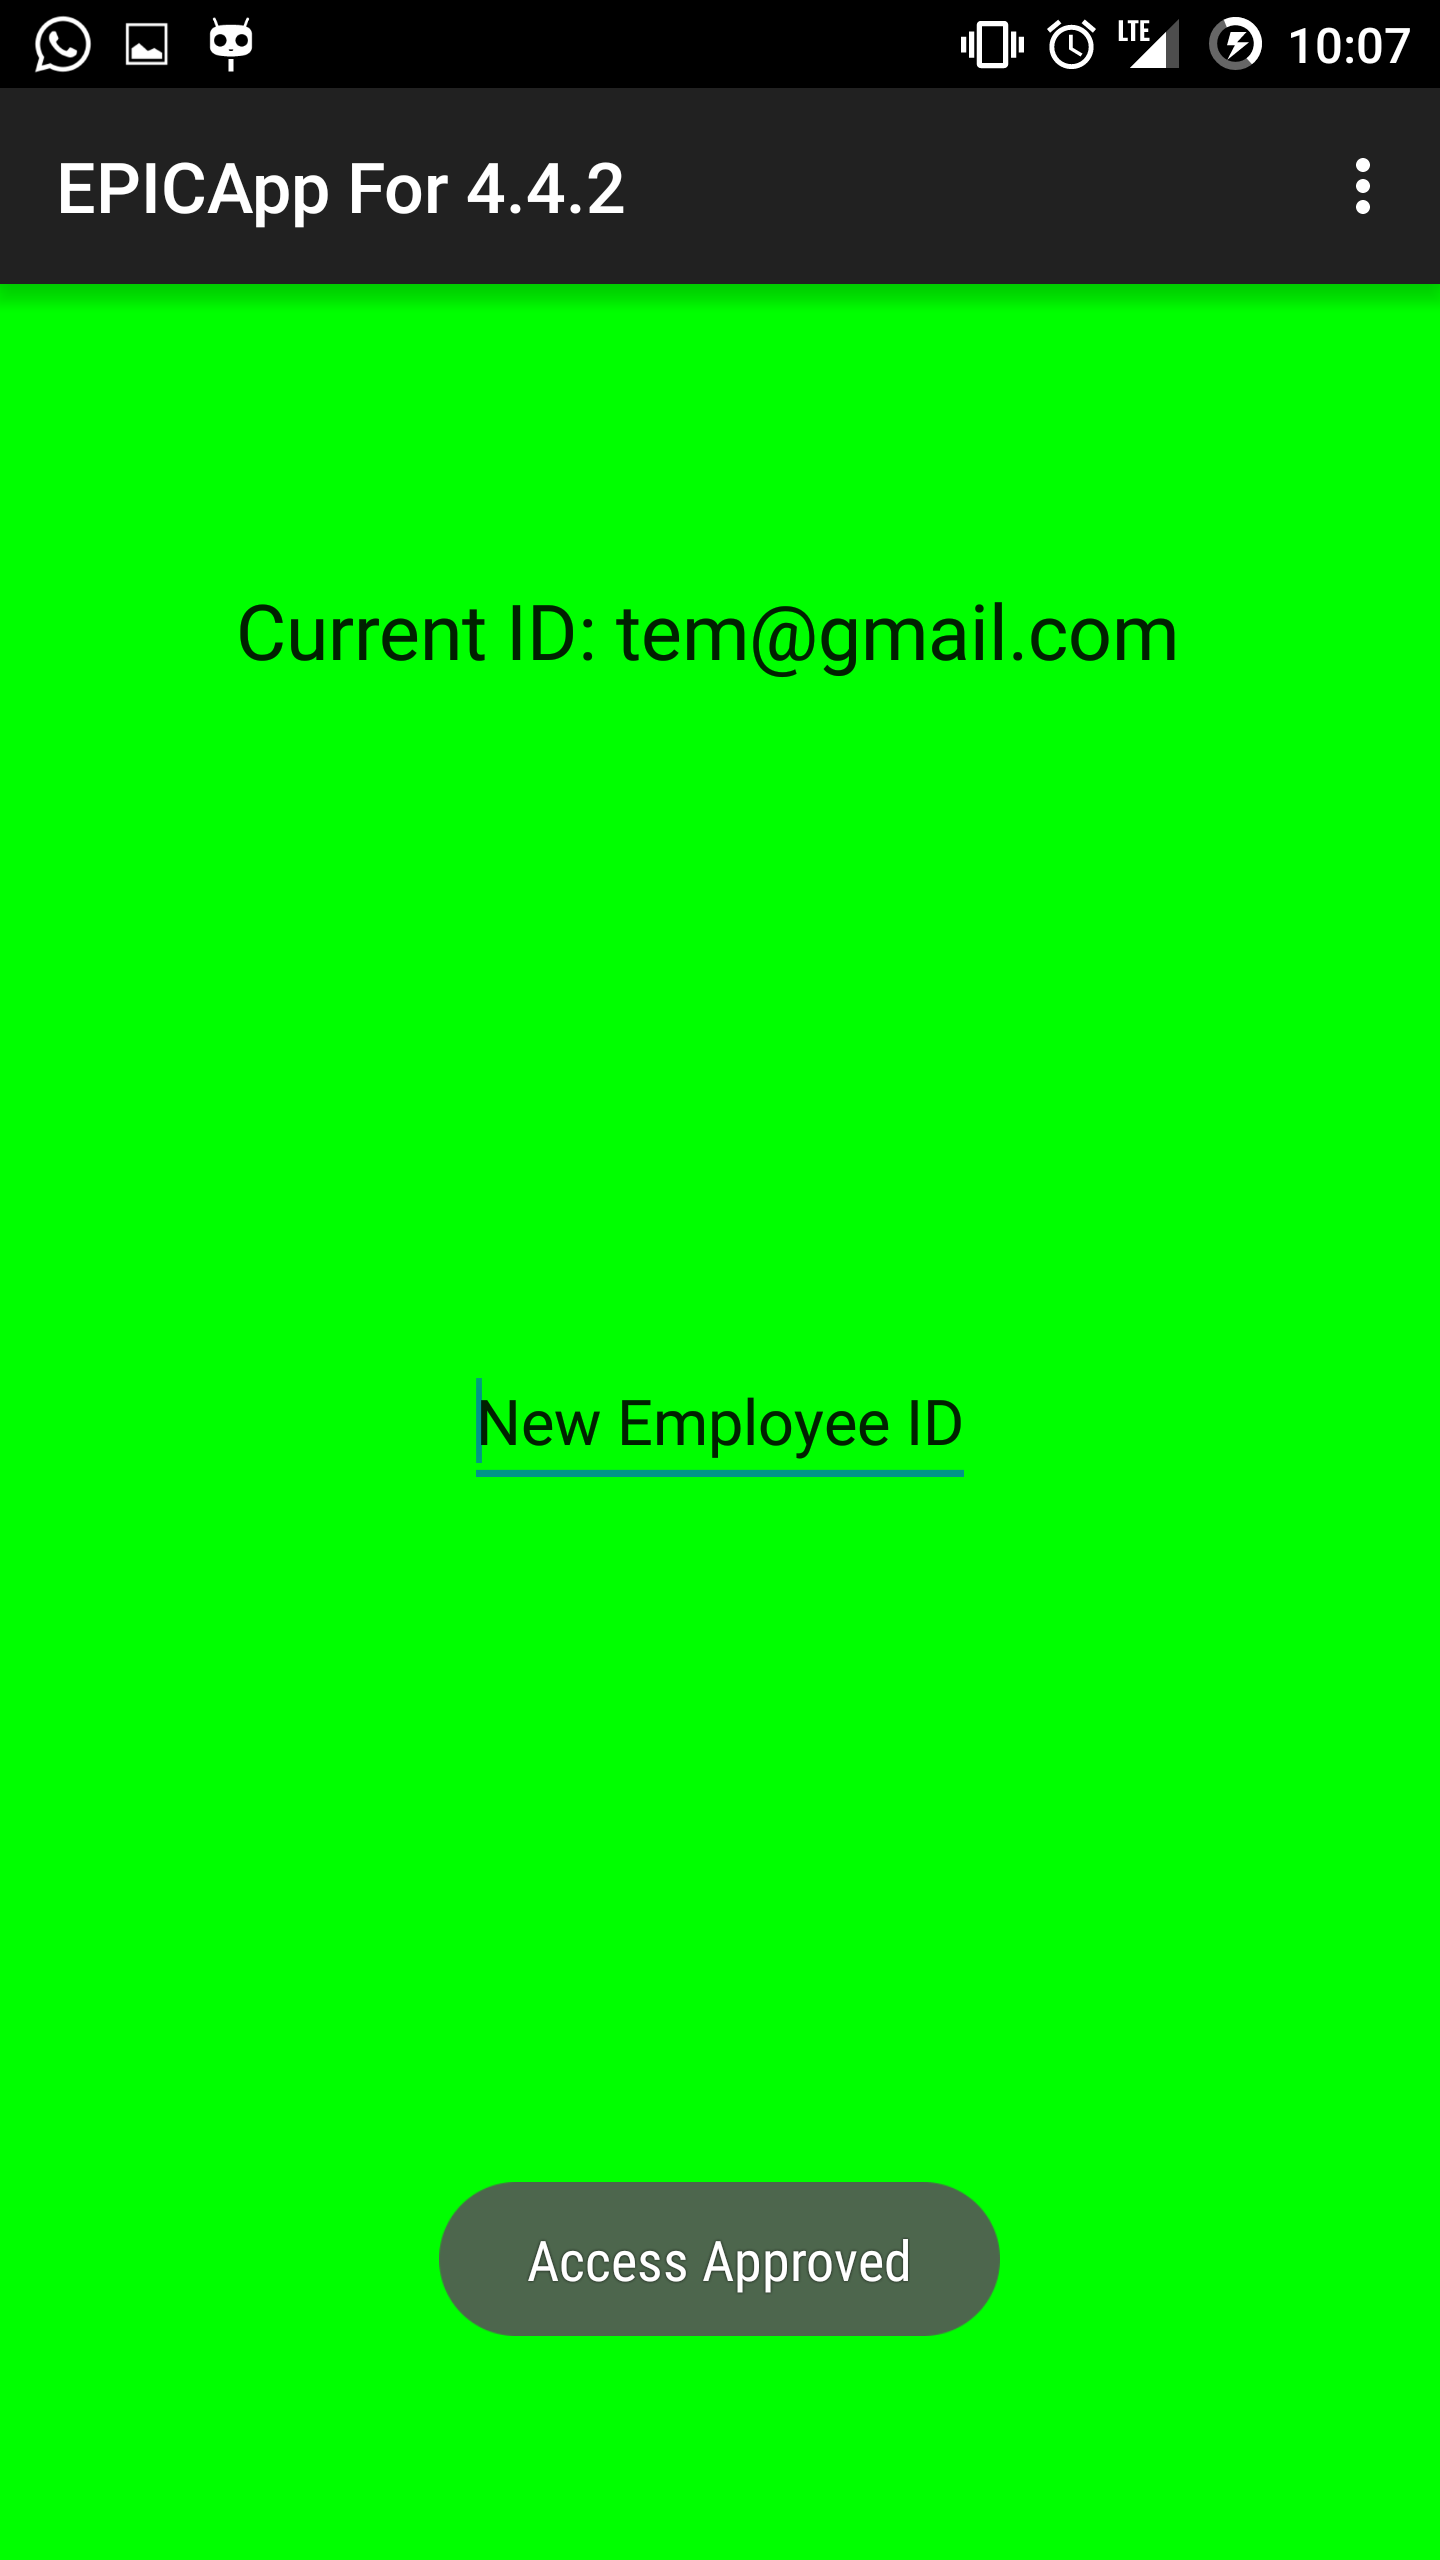
\includegraphics[width=5cm, height=6cm]{Approved}
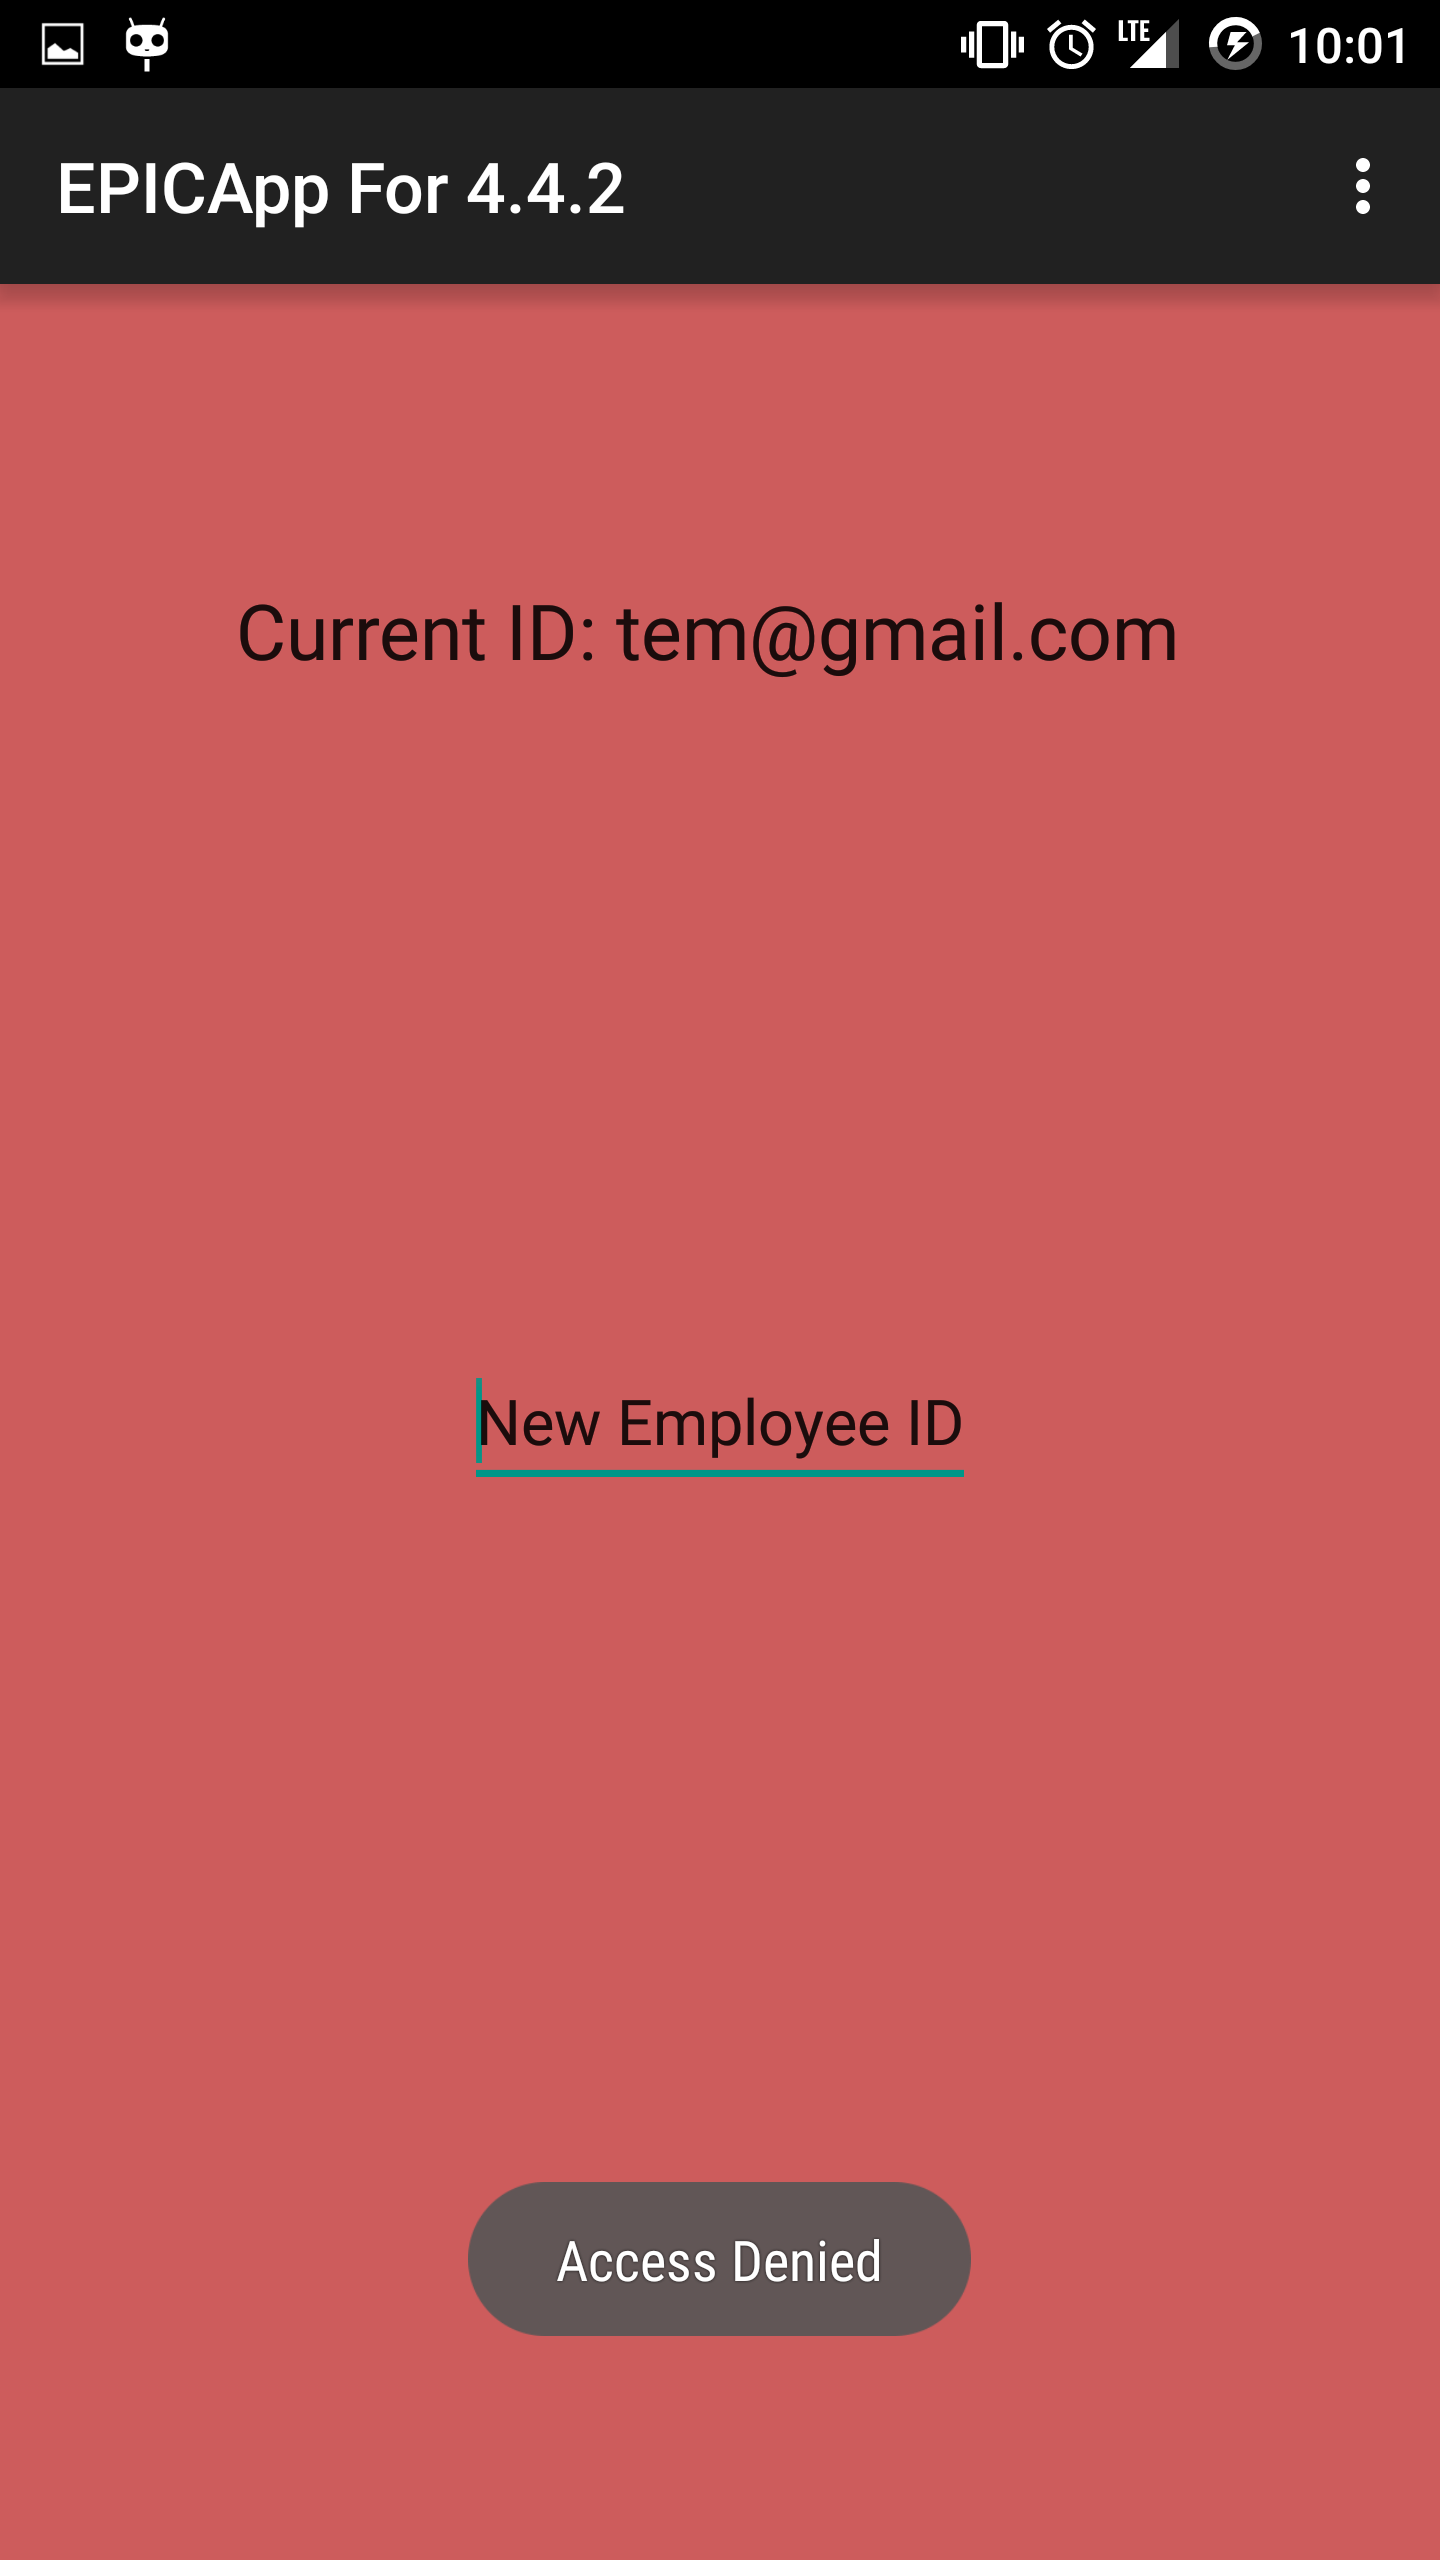
\includegraphics[width=5cm, height=6cm]{Denied}
\caption{Approved and denied screens}
\label{fig:my_label3}
\end{figure}}
For green flash go to step 3 and for red flash go to step 4.
\item{You have gained access to the door and may enter or leave the room. Entering will turn communication channels off and leaving will turn them back on.}
\item{You have been denied access. Make sure you are at the correct meeting room and that you have been added to attend the meeting.}
\end{enumerate}
To change users follow these steps:
\begin{enumerate}
\item{ Screen there is an edit box with the text \textit{New Employee ID} or your current ID. Click on it and type in the registered ID given to you and press the done or check mark key.
\begin{figure}[H]
\center
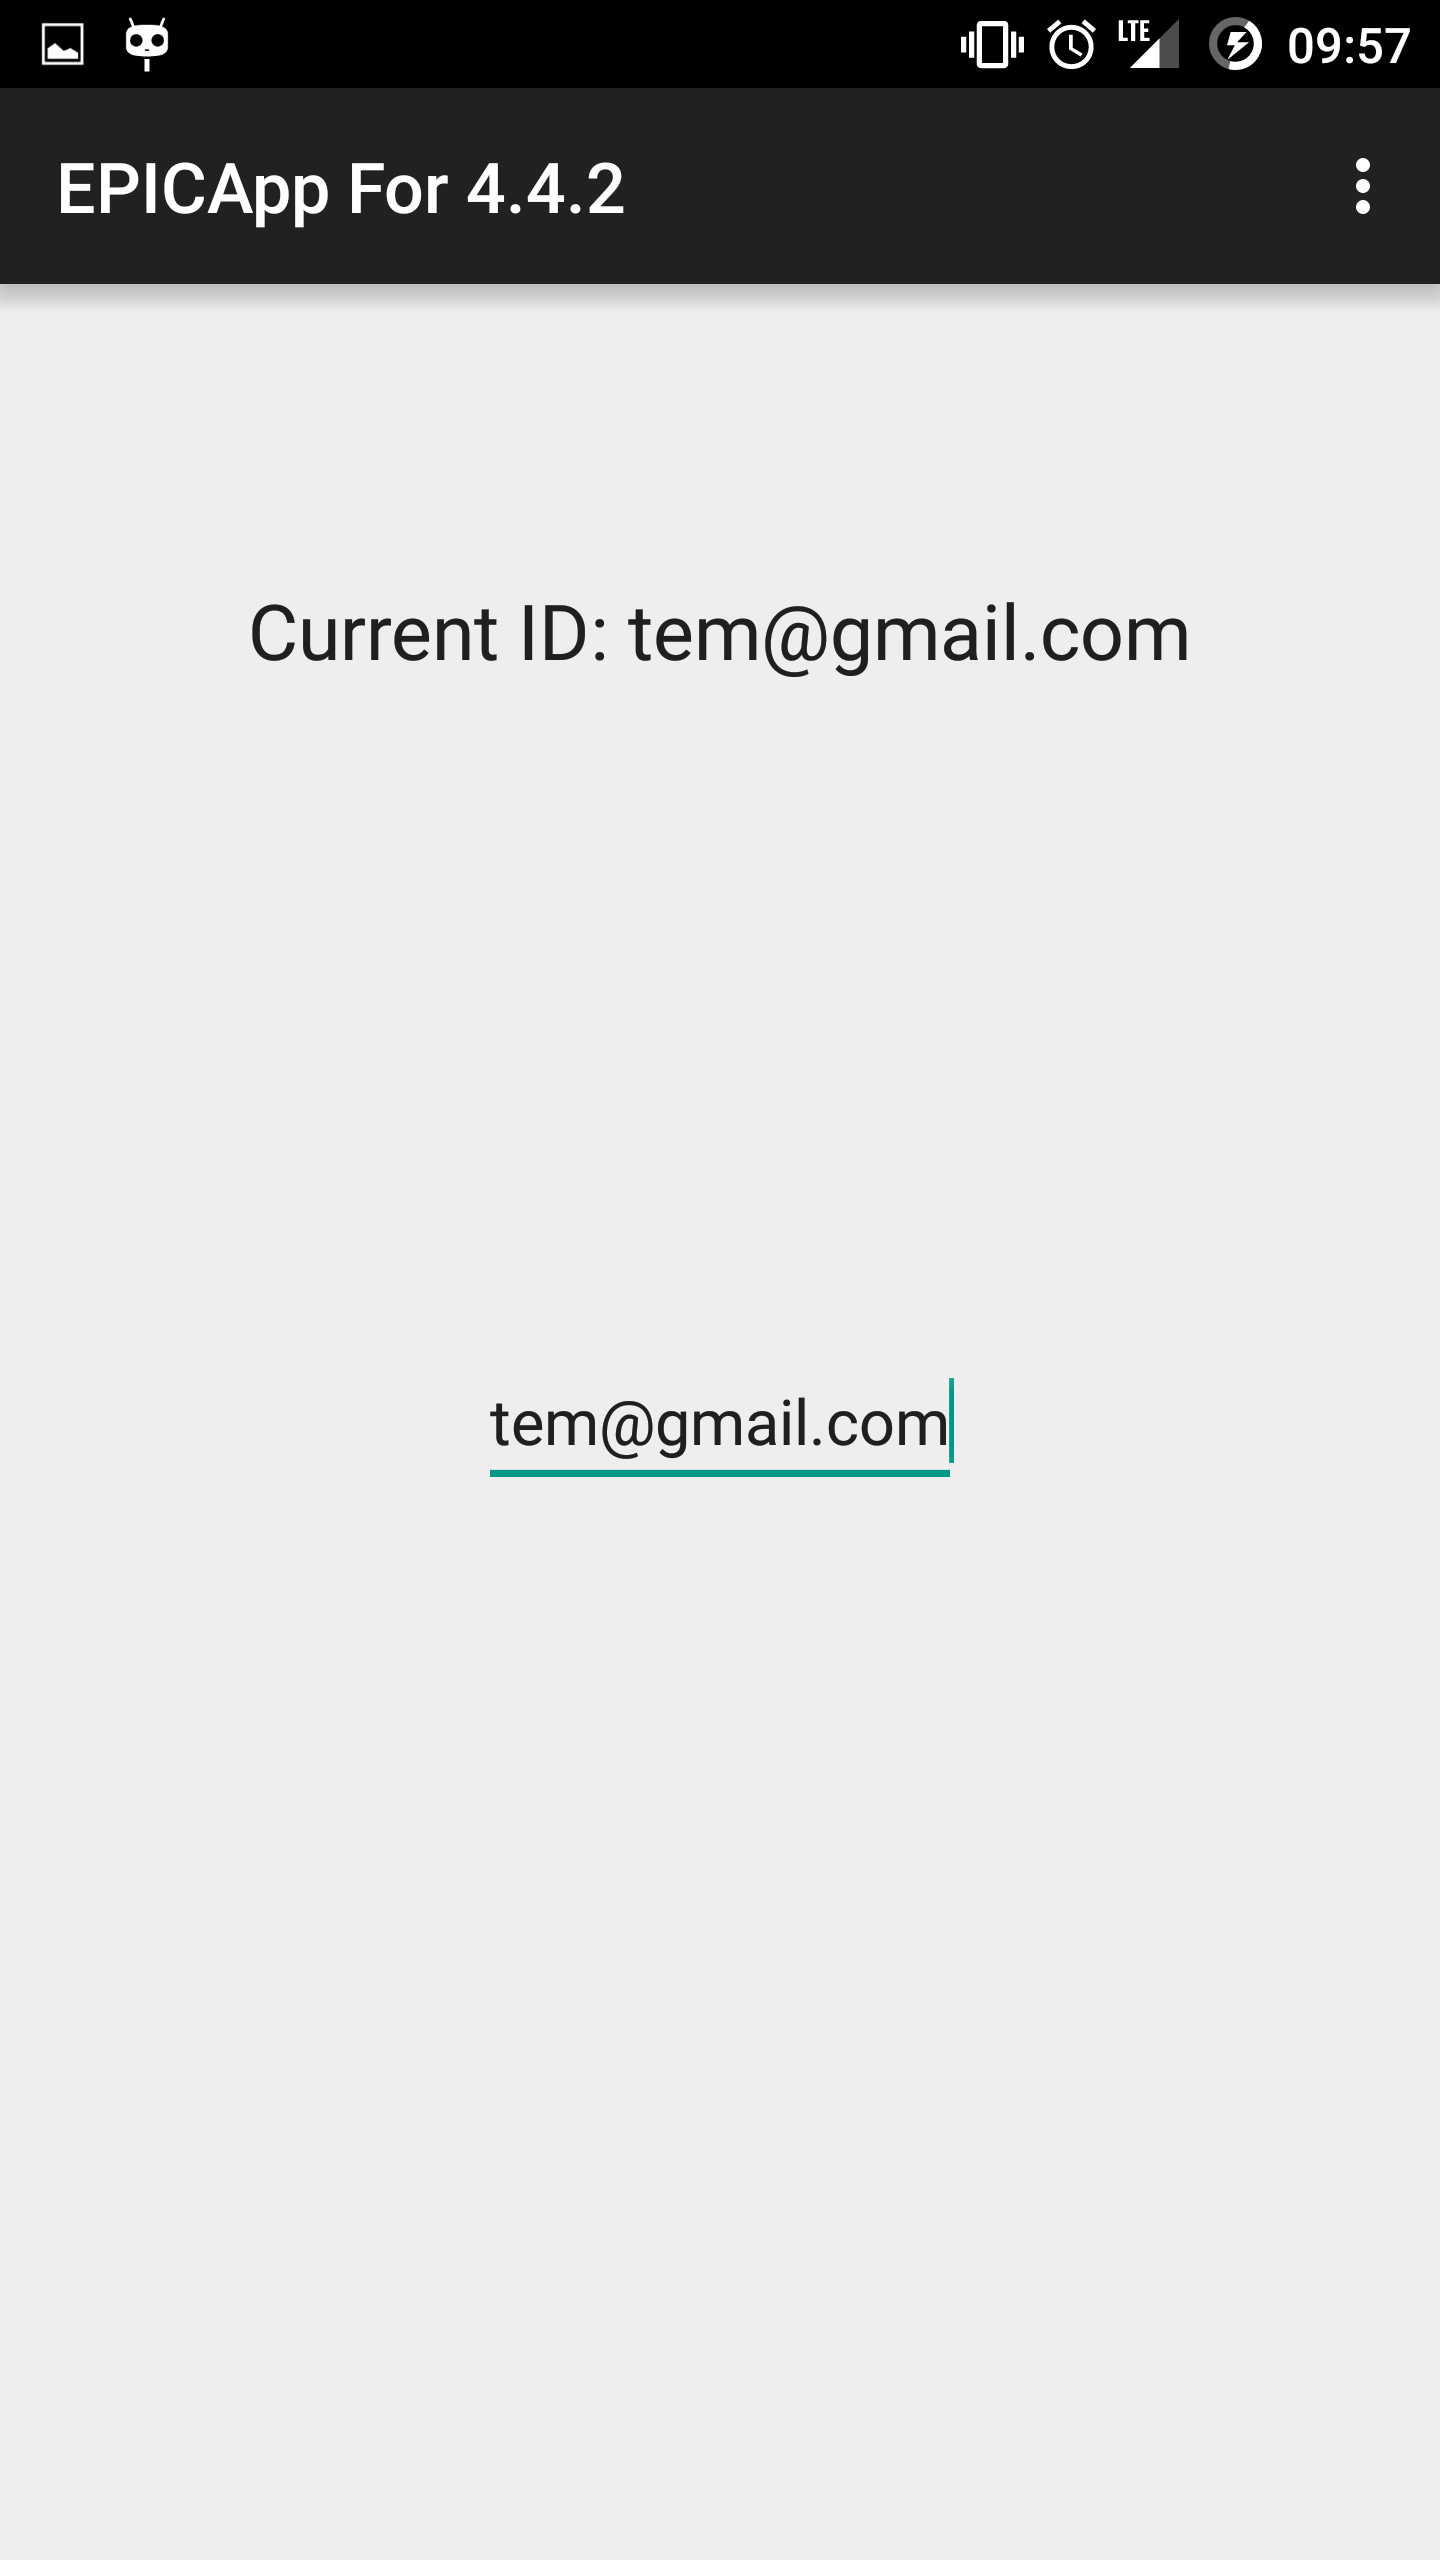
\includegraphics[width=5cm, height=6cm]{SecOpen}
\caption{Main Screen}
\label{fig:my_label4}
\end{figure}}
\item You will notice the text at the top change to your ID that you typed in. This means that the application is now ready to be used to enter and leave the meeting room.
\end{enumerate}

\subsection{Node}
If the Node is plugged in and functioning correctly, the lights should be Orange and Yellow strips running across. If this isn't the case, see the Troubleshooting section of this document.

The Node has the following states:
\begin{itemize}
\item When the lights are Orange and Yellow strips running across, the Node is in the ready and waiting state.
\item When the lights have a Blue bar counting up and a White light running back and forth, the Node is in the processing state.
\item When all the lights are Red, the Server has denied your request for entering the meeting.
\item When all the lights are Green, the Server has approved your request for entering the meeting.
\item When all the lights are Orange, somewhere something went wrong.
\end{itemize}
Here is what you can do and when:
\begin{itemize}
\item In the ready and waiting state you can place your phone on the Node with the protection app open.
\item In the processing state you must leave your phone on the node.
\item When the lights have either turned Green, Red or Orange, you can remove your phone from the Node.
\end{itemize}

\subsection{Website}
    \begin{itemize}
        \item If you want to register, open \url{http://projectepic.info/register} in your favourite web browser. Type your details in and click on the "register" button. After you have registered, you will automatically be logged in. It will look like this: 
        \begin{figure}[H]
                \centering
                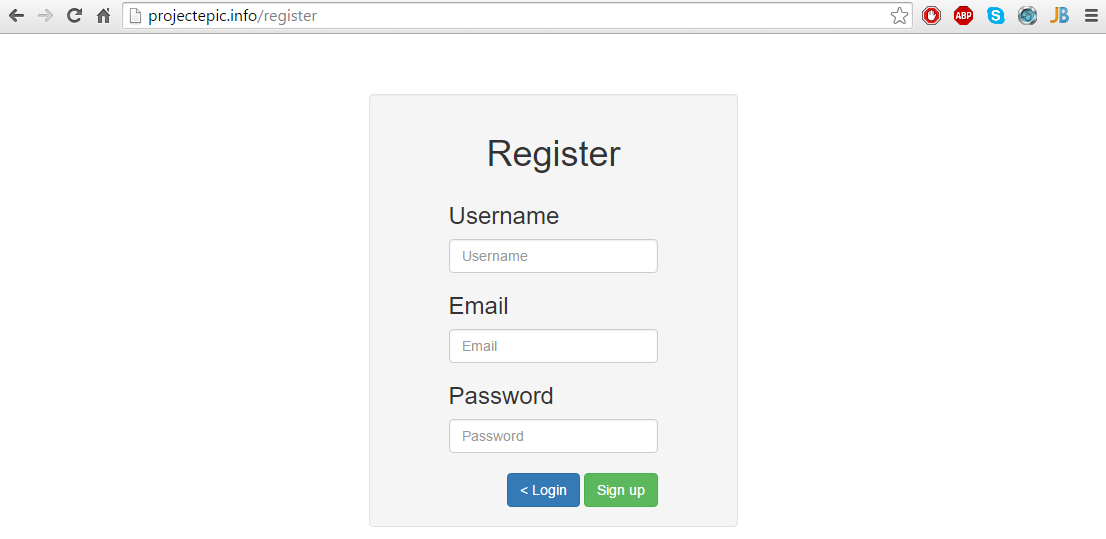
\includegraphics[width=10cm]{webPics/register}
                \caption{Website Register Page}
                \label{fig}
            \end{figure}       
        \item {If you have registered, you may log in at \url{http://projectepic.info/login}. Simply type in your details and then you may log in by pressing the "Log in" button. You may also log in via Facebook It will look like this: 
        \begin{figure}[H]
                \centering
                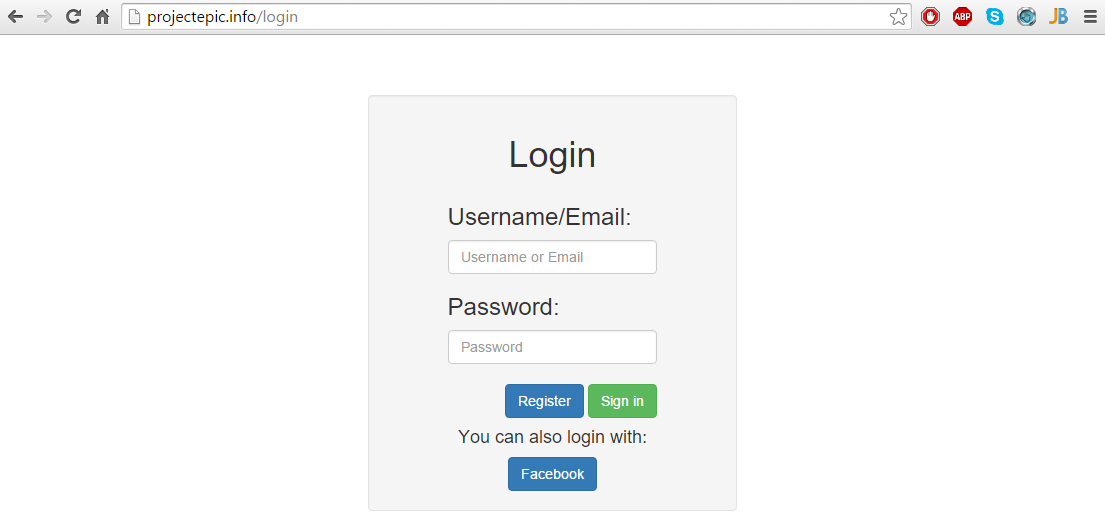
\includegraphics[width=10cm]{webPics/login}
                \caption{Website Login Page}
                \label{fig}
            \end{figure}}
        
        \item {To schedule a meeting you must redirect your browser to \url{http://projectepic.info/meetings}. You may then add another meeting by filling out the details. You may remove a meeting simply by clicking on the "Remove" button next to the meeting details. 
        \begin{figure}[H]
                \centering
                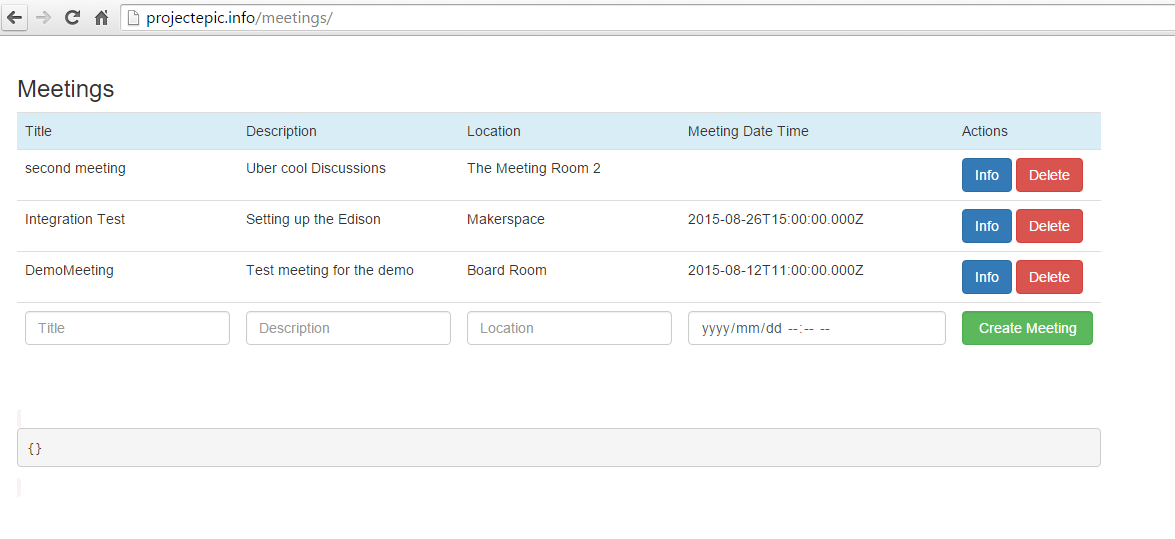
\includegraphics[width=10cm]{webPics/meetings}
                \caption{Website Meetings Page}
                \label{fig}
            \end{figure}}
            
            \item {If you wish to invite people to your meeting, click on the blue "Info" button next to the meeting. The list of invitees will then appear to the right. To invite people, type in their details in the fields and click on the "Invite" button. An invitation will then be send to them via email. You may also remove an invitee by clicking on the "Remove" button next to their name. 
          \begin{figure}[H]
                \centering
                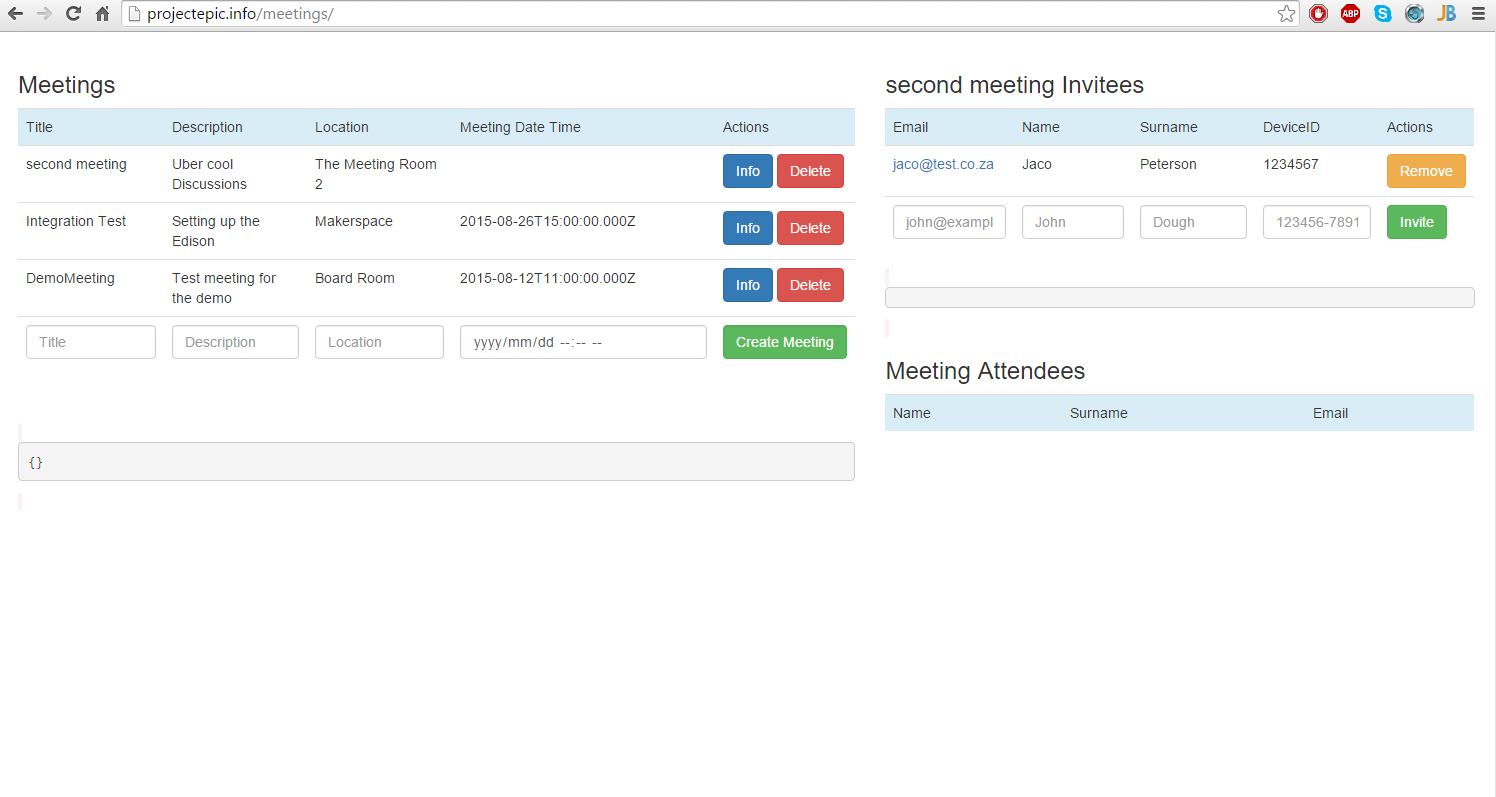
\includegraphics[width=10cm]{webPics/meetinginfo}
                \caption{Website Meeting Invitees Page}
                \label{fig}
            \end{figure}}          
            

\end{itemize}


\subsection{EPIC Malware}
\subsubsection{Java Malware Server}
\begin{itemize}
\item{If application control is selected the server waits for an incoming connection and starts recording. Using this option the android application is manually controlled. When local recording and streaming needs to be stopped select yes from the stop recording, dialog this will terminate and save the recording.
\begin{figure}[H]
\center
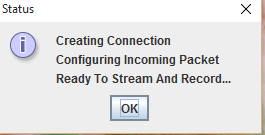
\includegraphics[width=5cm, height=3cm]{MalwareScreenshots/infoStatus}
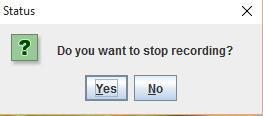
\includegraphics[width=5cm, height=3cm]{MalwareScreenshots/stopRec}
\caption{Malware Server options}
\label{fig:my_label7}
\end{figure}}
\item{If server control is selected the server will wait for incoming requests to connect to the server and add them to a list. 
\begin{figure}[H]
\center
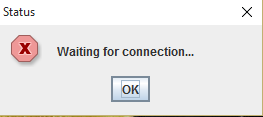
\includegraphics[width=8cm, height=3cm]{MalwareScreenshots/waiting}
\caption{Malware Server server control option selected}
\label{fig:my_label8}
\end{figure}
The user will be able to select a device from the list to eavesdrop on.
\begin{figure}[H]
\center
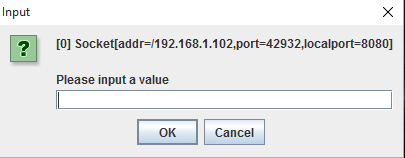
\includegraphics[width=8cm, height=5cm]{MalwareScreenshots/select}
\caption{Malware Server device list}
\label{fig:my_label9}
\end{figure}
When a device is selected from the list the server will start to record the incoming stream. When the you want to stop the recording select yes from the stop recording dialog and the server will terminate and save a local recoding of the stream.
\begin{figure}[H]
\center
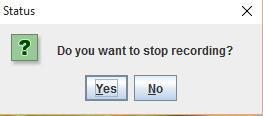
\includegraphics[width=5cm, height=3cm]{MalwareScreenshots/stopRec}
\caption{Malware Server recording from device}
\label{fig:my_label10}
\end{figure}}
\end{itemize}
\subsubsection{Android Malware Application}
The android application can only be manually controlled when application control is selected on the malware server.
When the start recording button is pressed the audio stream will be sent to the server. The start recording button is now greyed out.
\begin{figure}[H]
\center
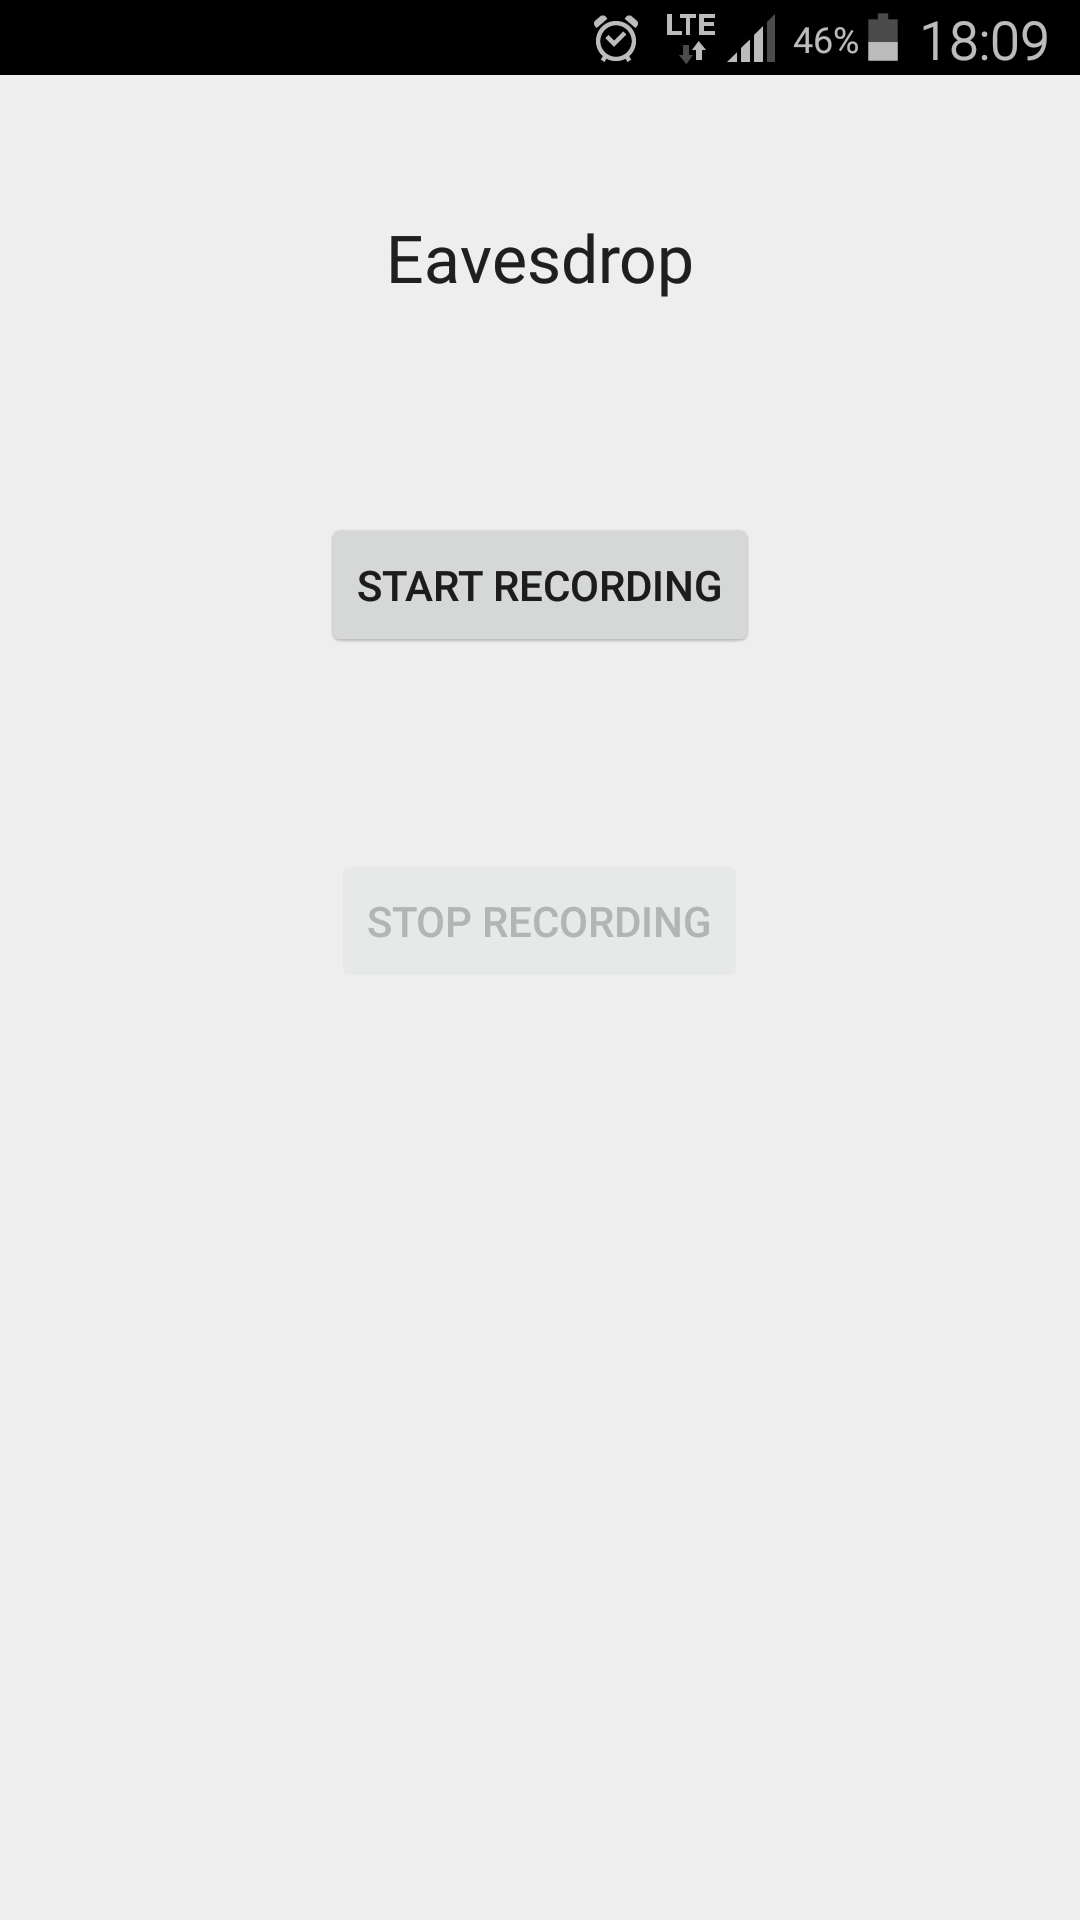
\includegraphics[width=5cm, height=6cm]{MalwareScreenshots/StartRecording}
\caption{Android malware application start recording}
\label{fig:my_label11}
\end{figure}
When the stop recording button is pressed the application stops to send a audio stream to the server. The user must also stop the server to save a copy of the stream on the device running the server.
\begin{figure}[H]
\center
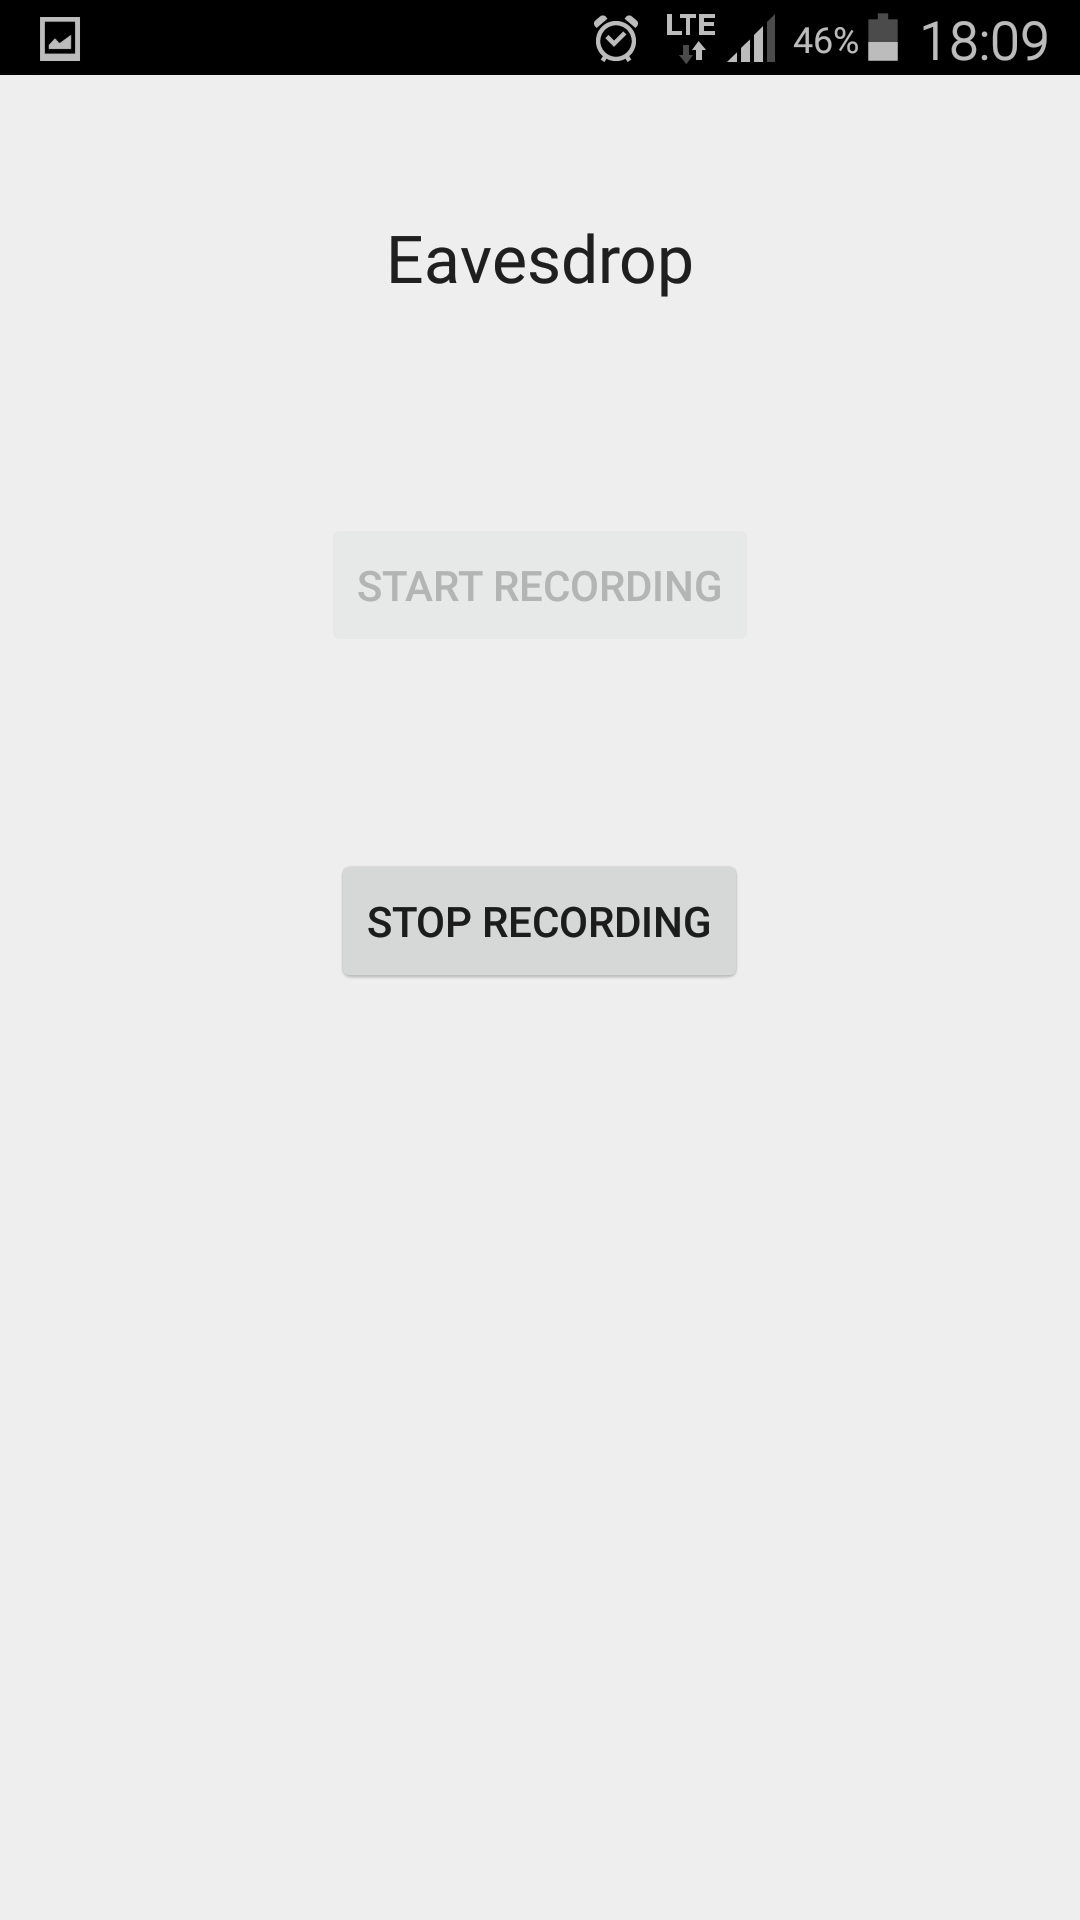
\includegraphics[width=5cm, height=6cm]{MalwareScreenshots/StopRecording}
\caption{Android malware application stop recording}
\label{fig:my_label12}
\end{figure}



\newpage
\section{Troubleshooting}
\subsection{Android Application}
\begin{itemize}
\item If you cannot find the application on the store it means that you either do not have the correct Android Operating System(4.4), your device doesn't have NFC or your device doesn't support HCE(Host Card Emulation). Please consult your device's manual.
\item If the application is not scanning (changing colour), check that NFC is enabled.
\item If you cannot access a room that you should have access to, make sure that you spelling of your employee ID is correct (the system is case sensitive). Also confirm that you have been added to the meeting.
\end{itemize}

\subsection{Node}
\begin{itemize}
\item If the lights turn Orange after you scanned your phone, you can check the Server or Gateway for error codes.
\item If the lights freeze or go off completely and the problem doesn't go away after a few seconds, you can either plug it out and in again or check what caused this on the Gateway.
\end{itemize}


\subsection{Website}
\begin{itemize}
\item If the elements on the website overlap, adjust the size of the browser window.
\item If the button doesn't work, wait patiently for the project to finish.
\item If the server is not found, wait five minutes and try again.
\end{itemize}


\subsection{EPIC Malware}
\subsubsection{Java Malware Server}
\begin{itemize}
\item If the server cannot stream the audio or no devices are detected open ports 4545 and 8080 on your firewall. These ports are used for communication between the application and the server.
\end{itemize}
\subsubsection{Android Malware Application}
\begin{itemize}
\item If any problems occur within the application just restart the application.
\end{itemize}

\end{document}
